\documentclass[12pt,a4paper,twoside,openright]{report}
\let\openright=\cleardoublepage



%%% Choose a language %%%

\newif\ifEN
\ENtrue   % uncomment this for english
%\ENfalse   % uncomment this for czech

%%% Configuration of the title page %%%

\def\ThesisTitleStyle{mff} % MFF style
%\def\ThesisTitleStyle{cuni} % uncomment for old-style with cuni.cz logo
%\def\ThesisTitleStyle{natur} % uncomment for nature faculty logo

\def\UKFaculty{Faculty of Mathematics and Physics}
%\def\UKFaculty{Faculty of Science}

\def\UKName{Charles University in Prague} % this is not used in the "mff" style

% Thesis type names, as used in several places in the title
\def\ThesisTypeTitle{\ifEN BACHELOR THESIS \else BAKALÁŘSKÁ PRÁCE \fi}
%\def\ThesisTypeTitle{\ifEN MASTER THESIS \else DIPLOMOVÁ PRÁCE \fi}
%\def\ThesisTypeTitle{\ifEN RIGOROUS THESIS \else RIGORÓZNÍ PRÁCE \fi}
%\def\ThesisTypeTitle{\ifEN DOCTORAL THESIS \else DISERTAČNÍ PRÁCE \fi}
\def\ThesisGenitive{\ifEN bachelor \else bakalářské \fi}
%\def\ThesisGenitive{\ifEN master \else diplomové \fi}
%\def\ThesisGenitive{\ifEN rigorous \else rigorózní \fi}
%\def\ThesisGenitive{\ifEN doctoral \else disertační \fi}
\def\ThesisAccusative{\ifEN bachelor \else bakalářskou \fi}
%\def\ThesisAccusative{\ifEN master \else diplomovou \fi}
%\def\ThesisAccusative{\ifEN rigorous \else rigorózní \fi}
%\def\ThesisAccusative{\ifEN doctoral \else disertační \fi}



%%% Fill in your details %%%

% (Note: \xxx is a "ToDo label" which makes the unfilled visible. Remove it.)
\def\ThesisTitle{\xxx{Thesis title}}
\def\ThesisAuthor{\xxx{Your Name Surname}}
\def\YearSubmitted{\xxx{YEAR}}

% department assigned to the thesis
\def\Department{\xxx{Name of the department}}
% Is it a department (katedra), or an institute (ústav)?
\def\DeptType{\xxx{Department}}

\def\Supervisor{\xxx{Supername Supersurname}}
\def\SupervisorsDepartment{\xxx{department}}

% Study programme and specialization
\def\StudyProgramme{\xxx{study programme}}
\def\StudyBranch{\xxx{study branch}}

\def\Dedication{%
Dedication. \xxx{It is nice to say thanks to supervisors, friends, family, book authors and food providers.}
}

\def\AbstractEN{%
\xxx{Abstracts are an abstract form of art. Use the most precise, shortest sentences that state what problem the thesis addresses, how it is approached, pinpoint the exact result achieved, and describe the applications and significance of the results. Highlight anything novel that was discovered or improved by the thesis. Maximum length is 200 words, but try to fit into 120. Abstracts are often used for deciding if a reviewer will be suitable for the thesis; a well-written abstract thus increases the probability of getting a reviewer who will like the thesis.}
% ABSTRACT IS NOT A COPY OF YOUR THESIS ASSIGNMENT!
}

\def\AbstractCS{%
\xxx{You will need to submit both Czech and English abstract to the SIS, no matter what language you use in the thesis. If writing in English, translate the contents of \texttt{\textbackslash{}AbstractEN} into this field. In case you do not speak czech, your supervisor should be able to help you with the translation.}
}

% 3 to 5 keywords (recommended), each enclosed in curly braces.
% Keywords are useful for indexing and searching for the theses by topic.
\def\Keywords{%
\xxx{{key} {words}}
}

% If your abstracts are long and do not fit in the infopage, you can make the
% fonts a bit smaller by this setting. (Also, you should try to compress your abstract more.)
% Alternatively, consider increasing the size of the page by uncommenting the
% geometry modification in thesis.tex.
\def\InfoPageFont{}
%\def\InfoPageFont{\small}  %uncomment to decrease font size

\ifEN\relax\else
% If you are writing a czech thesis, you additionally need to fill in the
% english translation of the metadata here!
\def\ThesisTitleEN{\xxx{Thesis title in English}}
\def\DepartmentEN{\xxx{Name of the department in English}}
\def\DeptTypeEN{\xxx{Department}}
\def\SupervisorsDepartmentEN{\xxx{Superdepartment}}
\def\StudyProgrammeEN{\xxx{study programme}}
\def\StudyBranchEN{\xxx{study branch}}
\def\KeywordsEN{%
\xxx{{key} {words}}
}
\fi


\usepackage[a-2u]{pdfx}

\ifEN\else\usepackage[czech,shorthands=off]{babel}\fi
\usepackage[utf8]{inputenc}
\usepackage[T1]{fontenc}

% See https://en.wikipedia.org/wiki/Canons_of_page_construction before
% modifying the size of printable area. LaTeX defaults are great.
% If you feel it would help anything, you can enlarge the printable area a bit:
%\usepackage[textwidth=390pt,textheight=630pt]{geometry}
% The official recommendation expands the area quite a bit (looks pretty harsh):
%\usepackage[textwidth=145mm,textheight=247mm]{geometry}

%%% FONTS %%%
\usepackage{lmodern} % TeX "original" (this sets up the latin mono)

% Optionally choose an override for the main font for typesetting:
\usepackage[mono=false]{libertinus} % popular for comp-sci (ACM uses this)
%\usepackage{tgschola} % Schoolbook-like (gives a bit of historic feel)
%\usepackage[scale=0.96]{tgpagella} % Palladio-like (popular in formal logic).
% IBM Plex font suite is nice but requires us to fine-tune the sizes, also note
% that it does not directly support small caps (\textsc) and requires lualatex:
%\usepackage[usefilenames,RM={Scale=0.88},SS={Scale=0.88},SScon={Scale=0.88},TT={Scale=0.88},DefaultFeatures={Ligatures=Common}]{plex-otf}

% Optionally, choose a custom sans-serif fonts (e.g. for figures and tables).
% Default sans-serif font is usually Latin Modern Sans. Some font packages
% (e.g. libertinus) replace that with a better matching sans-serif font.
%\usepackage{tgheros} % recommended and very readable (Helvetica-like)
%\usepackage{FiraSans} % looks great
% DO NOT typeset the main text in sans-serif font!
% The serifs make the text easily readable on the paper.


% IMPORTANT FONT NOTE: Some fonts require additional PDF/A conversion using
% the pdfa.sh script. These currently include only 'tgpagella'; but various
% other fonts from the texlive distribution need that too (mainly the Droid
% font family).


% some useful packages
\usepackage{microtype}
\usepackage{amsmath,amsfonts,amsthm,bm}
\usepackage{graphicx}
\usepackage{xcolor}
\usepackage{booktabs}
\usepackage{caption}
\usepackage{floatrow}

% load bibliography tools
\usepackage[backend=bibtex,natbib,style=numeric,sorting=none]{biblatex}
% alternative with alphanumeric citations (more informative than numbers):
%\usepackage[backend=bibtex,natbib,style=alphabetic]{biblatex}
%
% alternatives that conform to iso690
% (iso690 is not formally required on MFF, but may help elsewhere):
%\usepackage[backend=bibtex,natbib,style=iso-numeric,sorting=none]{biblatex}
%\usepackage[backend=bibtex,natbib,style=iso-alphabetic]{biblatex}
%
% additional option choices:
%  - add `giveninits=true` to typeset "E. A. Poe" instead of full Edgar Allan
%  - `terseinits=true` additionaly shortens it to nature-like "Poe EA"
%  - add `maxnames=10` to limit (or loosen) the maximum number of authors in
%    bibliography entry before shortening to `et al.` (useful when referring to
%    book collections that may have hundreds of authors)
%  - for additional flexibility (e.g. multiple reference sections, etc.),
%    remove `backend=bibtex` and compile with `biber` instead of `bibtex` (see
%    Makefile)
%  - `sorting=none` causes the bibliography list to be ordered by the order of
%    citation as they appear in the text, which is usually the desired behavior
%    with numeric citations. Additionally you can use a style like
%    `numeric-comp` that compresses the long lists of citations such as
%    [1,2,3,4,5,6,7,8] to simpler [1--8]. This is especially useful if you plan
%    to add tremendous amounts of citations, as usual in life sciences and
%    bioinformatics.
%  - if you don't like the "In:" appearing in the bibliography, use the
%    extended style (`ext-numeric` or `ext-alphabetic`), and add option
%    `articlein=false`.
%
% possibly reverse the names of the authors with the default styles:
%\DeclareNameAlias{default}{family-given}

% load the file with bibliography entries
\addbibresource{refs}

% remove this if you won't use fancy verbatim environments
\usepackage{fancyvrb}

% remove this if you won't typeset TikZ graphics
\usepackage{tikz}
\usetikzlibrary{positioning} %add libraries as needed (shapes, decorations, ...)

% remove this if you won't typeset any pseudocode
\usepackage{algpseudocode}
\usepackage{algorithm}

% remove this if you won't list any source code
\usepackage{listings}


\hypersetup{unicode}
\hypersetup{breaklinks=true}

\usepackage[noabbrev]{cleveref}


% various forms of TODOs (you should remove this before submitting)
\usepackage[textsize=tiny, backgroundcolor=yellow!25, linecolor=black!25]{todonotes}
\newcommand{\xxx}[1]{\textcolor{red!}{#1}}

 % remove this before compiling the final version


% use this for typesetting a chapter without a number, e.g. intro and outro
\def\chapwithtoc#1{\chapter*{#1}\addcontentsline{toc}{chapter}{#1}}

% If there is a line/figure overflowing into page margin, this will make the
% problem evident by drawing a thick black line at the overflowing spot. You
% should not disable this.
\overfullrule=3mm

% The maximum stretching of a space. Increasing this makes the text a bit more
% sloppy, but may prevent the overflows by moving words to next line.
\emergencystretch=1em

\ifEN
\theoremstyle{plain}
\newtheorem{thm}{Theorem}
\newtheorem{lemma}[thm]{Lemma}
\newtheorem{claim}[thm]{Claim}
\newtheorem{defn}{Definition}
\theoremstyle{remark}
\newtheorem*{cor}{Corollary}
\else
\theoremstyle{plain}
\newtheorem{thm}{Věta}
\newtheorem{lemma}{Lemma}
\newtheorem{claim}{Tvrzení}
\newtheorem{defn}{Definice}
\theoremstyle{remark}
\newtheorem*{cor}{Důsledek}
\fi

\newenvironment{myproof}{
  \par\medskip\noindent
  \textit{\ifEN Proof \else Důkaz \fi}.
}{
\newline
\rightline{$\qedsymbol$}
}

% real/natural numbers
\newcommand{\R}{\mathbb{R}}
\newcommand{\N}{\mathbb{N}}

% asymptotic complexity
\newcommand{\asy}[1]{\mathcal{O}(#1)}

% listings and default lstlisting config (remove if unused)
\DeclareNewFloatType{listing}{}
\floatsetup[listing]{style=ruled}

\DeclareCaptionStyle{thesis}{style=base,font={small,sf},labelfont=bf,labelsep=quad}
\captionsetup{style=thesis}
\captionsetup[algorithm]{style=thesis,singlelinecheck=off}
\captionsetup[listing]{style=thesis,singlelinecheck=off}

% Customization of algorithmic environment (comment style)
\renewcommand{\algorithmiccomment}[1]{\textcolor{black!25}{\dotfill\sffamily\itshape#1}}

% Uncomment for table captions on top. This is sometimes recommended by the
% style guide, and even required for some publication types.
%\floatsetup[table]{capposition=top}
%
% (Opinionated rant:) Captions on top are not "compatible" with the general
% guideline that the tables should be formatted to be quickly visually
% comprehensible and *beautiful* in general (like figures), and that the table
% "head" row (with column names) should alone communicate most of the content
% and interpretation of the table. If you just need to show a long boring list
% of numbers (because you have to), either put some effort into showing the
% data in an attractive figure-table, or move the data to an attachment and
% refer to it, so that the boredom does not impact the main text flow.
%
% You can make the top-captions look much less ugly by aligning the widths of
% the caption and the table, with setting `framefit=yes`, as shown below.  This
% additionally requires some extra markup in your {table} environments; see the
% comments in the example table in `ch2.tex` for details.
%\floatsetup[table]{capposition=top,framefit=yes}

\ifEN\floatname{listing}{Listing}
\else\floatname{listing}{Výpis kódu}\fi
\lstset{ % use this to define styling for any other language
  language=C++,
  tabsize=2,
  showstringspaces=false,
  basicstyle=\footnotesize\tt\color{black!75},
  identifierstyle=\bfseries\color{black},
  commentstyle=\color{green!50!black},
  stringstyle=\color{red!50!black},
  keywordstyle=\color{blue!75!black}}

% Czech versions of the used cleveref references (It's not as convenient as in
% English because of declension, cleveref is limited to sg/pl nominative. Use
% plain \ref to dodge that.)
\ifEN\relax\else
\crefname{chapter}{kapitola}{kapitoly}
\Crefname{chapter}{Kapitola}{Kapitoly}
\crefname{section}{sekce}{sekce}
\Crefname{section}{Sekce}{Sekce}
\crefname{subsection}{sekce}{sekce}
\Crefname{subsection}{Sekce}{Sekce}
\crefname{subsubsection}{sekce}{sekce}
\Crefname{subsubsection}{Sekce}{Sekce}
\crefname{figure}{obrázek}{obrázky}
\Crefname{figure}{Obrázek}{Obrázky}
\crefname{table}{tabulka}{tabulky}
\Crefname{table}{Tabulka}{Tabulky}
\crefname{listing}{výpis}{výpisy}
\Crefname{listing}{Výpis}{Výpisy}
\floatname{algorithm}{Algoritmus}
\crefname{algorithm}{algoritmus}{algoritmy}
\Crefname{algorithm}{Algoritmus}{Algoritmy}
\newcommand{\crefpairconjunction}{ a~}
\newcommand{\crefrangeconjunction}{ a~}
\fi
 % use this file for various custom definitions


\begin{document}

% the layout is mandatory, edit only in dire circumstances

\pagestyle{empty}
\hypersetup{pageanchor=false}
\begin{center}

% top part of the layout, this actually differs between faculties

\def\ThesisTitleXmff{%
  \ifEN
    \centerline{\mbox{
\includegraphics[width=166mm]{img/logo-en.pdf}}}
  \else
    \centerline{\mbox{
\includegraphics[width=166mm]{img/logo-cs.pdf}}}
  \fi
  \vspace{-8mm}\vfill%
  {\bf\Large\ThesisTypeTitle}
  \vfill%
  {\LARGE\ThesisAuthor}\par
  \vspace{15mm}%
  {\LARGE\bfseries\ThesisTitle}
  \vfill%
  \Department}
\def\ThesisTitleCuniLogo#1{%
  {\large\UKName\par\medskip\par\UKFaculty }
  \vfill%
  {\bf\Large\ThesisTypeTitle}
  \vfill%
  \includegraphics[width=70mm]{#1}
  \vfill%
  {\LARGE\ThesisAuthor}\par
  \vspace{15mm}%
  {\LARGE\bfseries\ThesisTitle}
  \vfill%
  \Department\par}
\def\ThesisTitleXcuni{\ThesisTitleCuniLogo{img/uklogo.pdf}}
\def\ThesisTitleXnatur{\ThesisTitleCuniLogo{img/naturlogo.pdf}}

% choose the correct page and print it
\csname ThesisTitleX\ThesisTitleStyle\endcsname
% latex corner: X is the new @

\vfill

{
\centerline{\vbox{\halign{\hbox to 0.45\hsize{\hfil #}&\hskip 0.5em\parbox[t]{0.45\hsize}{\raggedright #}\cr
\ifEN Supervisor of the \ThesisGenitive thesis:
\else Vedoucí \ThesisGenitive práce: \fi
& \Supervisor \cr
\noalign{\vspace{2mm}}
\ifEN Study programme: \else Studijní program: \fi
& \StudyProgramme \cr
\noalign{\vspace{2mm}}
\ifEN Study branch: \else Studijní obor: \fi
& \StudyBranch \cr
}}}}

\vfill

\ifEN Prague \else Praha \fi
\YearSubmitted

\end{center}

\newpage

% remember to sign this!
\openright
\hypersetup{pageanchor=true}
\pagestyle{plain}
\pagenumbering{roman}
\vglue 0pt plus 1fill

\ifEN
\noindent
I declare that I carried out this \ThesisAccusative thesis independently, and only with the cited
sources, literature and other professional sources. It has not been used to obtain another
or the same degree.
\else
\noindent
Prohlašuji, že jsem tuto \ThesisAccusative práci vypracoval(a) samostatně a výhradně
s~použitím citovaných pramenů, literatury a dalších odborných zdrojů.
Tato práce nebyla využita k získání jiného nebo stejného titulu.
\fi

\ifEN
\medskip\noindent
I understand that my work relates to the rights and obligations under the Act No.~121/2000 Sb.,
the Copyright Act, as amended, in particular the fact that the Charles
University has the right to conclude a license agreement on the use of this
work as a school work pursuant to Section 60 subsection 1 of the Copyright~Act.
\else
\medskip\noindent
Beru na~vědomí, že se na moji práci vztahují práva a povinnosti vyplývající
ze zákona č. 121/2000 Sb., autorského zákona v~platném znění, zejména skutečnost,
že Univerzita Karlova má právo na~uzavření licenční smlouvy o~užití této
práce jako školního díla podle §60 odst. 1 autorského zákona.
\fi

\vspace{10mm}


\ifEN
\hbox{\hbox to 0.5\hsize{%
In \hbox to 6em{\dotfill} date \hbox to 6em{\dotfill}
\hss}\hbox to 0.5\hsize{\dotfill\quad}}
\smallskip
\hbox{\hbox to 0.5\hsize{}\hbox to 0.5\hsize{\hfil Author's signature\hfil}}
\else
\hbox{\hbox to 0.5\hsize{%
V \hbox to 6em{\dotfill} dne \hbox to 6em{\dotfill}
\hss}\hbox to 0.5\hsize{\dotfill\quad}}
\smallskip
\hbox{\hbox to 0.5\hsize{}\hbox to 0.5\hsize{\hfil Podpis autora\hfil}}
\fi

\vspace{20mm}
\newpage

% dedication

\openright

\noindent
\Dedication

\newpage

% mandatory information page

\openright

\vbox to 0.49\vsize{\InfoPageFont
\setlength\parindent{0mm}
\setlength\parskip{5mm}

\ifEN Title: \else Název práce: \fi
\ThesisTitle

\ifEN Author: \else Autor: \fi
\ThesisAuthor

\DeptType:
\Department

\ifEN Supervisor: \else Vedoucí bakalářské práce: \fi
\Supervisor, \SupervisorsDepartment

\ifEN Abstract: \AbstractEN \else Abstrakt: \AbstractCS \fi

\ifEN Keywords: \else Klíčová slova: \fi
\Keywords

\vss}\ifEN\relax\else\nobreak\vbox to 0.49\vsize{\InfoPageFont
\setlength\parindent{0mm}
\setlength\parskip{5mm}

Title:
\ThesisTitleEN

Author:
\ThesisAuthor

\DeptTypeEN:
\DepartmentEN

Supervisor:
\Supervisor, \SupervisorsDepartmentEN

Abstract:
\AbstractEN

Keywords:
\KeywordsEN

\vss}
\fi

\newpage

\openright
\pagestyle{plain}
\pagenumbering{arabic}
\setcounter{page}{1}


\tableofcontents


\chapwithtoc{Introduction}

%%%%%%%%%%%%%%%%%%%%%%%%%%%%%%%%%%%%%%%%%%%%%%%%%%%%%%%%%%%%%%%%%%%%%%
% Introduction should answer the following questions, ideally in this order:
% \begin{enumerate}
% \item What is the nature of the problem the thesis is addressing?
% \item What is the common approach for solving that problem now?
% \item How this thesis approaches the problem?
% \item What are the results? Did something improve?
% \item What can the reader expect in the individual chapters of the thesis?
% \end{enumerate}
% 
% Expected length of the introduction is between 1--4 pages. Longer introductions may require sub-sectioning with appropriate headings --- use \texttt{\textbackslash{}section*} to avoid numbering (with section names like `Motivation' and `Related work'), but try to avoid lengthy discussion of anything specific. Any ``real science'' (definitions, theorems, methods, data) should go into other chapters.
% \todo{You may notice that this paragraph briefly shows different ``types'' of `quotes' in TeX, and the usage difference between a hyphen (-), en-dash (--) and em-dash (---).}
% 
% It is very advisable to skim through a book about scientific English writing before starting the thesis. I can recommend `\citetitle{glasman2010science}' by \citet{glasman2010science}.
% 
%%%%%%%%%%%%%%%%%%%%%%%%%%%%%%%%%%%%%%%%%%%%%%%%%%%%%%%%%%%%%%%%%%%


% adapted from the thesis assignment

Modern containerized cloud computing systems have complex requirements for their networking backends. Demand for features like seamless cross-data-center networking, multi-tenancy and security policies necessitated the use of the Software Defined Networking (SDN) concept and, by the nature of containerized systems, extensive use of virtualized networks.

The current shift to microservices and the resulting increase of endpoints and the need for rapid reconfiguration emphasized the SDN control plane performance and scalability.

A commonly deployed solution is Kubernetes for container orchestration and Open vSwitch for the virtualized SDN, used either directly or indirectly. However, it remains a question of how well these solutions are adapted to the networking needs of microservices.

This work explores the performance and scalability characteristics of Open vSwitch (OVS) based Kubernetes clusters and is focused on investigating performance in pathological scenarios. While our experimental Kubernetes clusters were configured with the OVN-Kubernetes networking plugin, our findings should be transferrable to any other SDN installation using Open vSwitch.

We explored methods for stressing the OVS's control plane and discovered several problematic traffic patterns. We measured OVS's behavior under stress and learned that in certain configurations, an attacker can use the discovered inefficiencies for an effective denial of service attack on the local cluster node.

This thesis is divided into several chapters. In the first chapter, we provide descriptions of all relevant technologies, how they interact and how they work internally. The second chapter describes the configuration of our experimental clusters to allow anyone to replicate our findings. We describe our experiments in chapter three and their results in chapter four. The fifth chapter is about our additional discoveries, and the last, sixth, chapter discusses the big picture of our findings. \todo{fix chapter descriptions when everything is finished}



% The rest of the assignment text:
%
% The goal of this work is exploring the performance and scalability of common Kubernetes and Open vSwitch configurations with the focus on pathological cases. It should explore how network performance characteristics are influenced by external factors, such as pathologic traffic patterns or pathologic microservices networking behavior. It should seek performance and scalability bottlenecks, evaluate whether and how they are relevant to the cluster security and propose optimization.

\chapter{Theoretical background}
\label{chap:refs}

\section{Glossary}

\paragraph{SDN} Software-defined network. Additional details can be found in \xxx{\cref{TODO}}.

\paragraph{OVS} Open vSwitch\footnote{\url{https://www.openvswitch.org/}}

\paragraph{OVN} Open Virtual Network\footnote{\url{https://docs.ovn.org/en/latest/}}

\paragraph{CNI} Container network interface\footnote{\url{https://github.com/containernetworking/cni/blob/dc0779e8cec8bfe39bc0d7a038250e233e5214eb/SPEC.md}}. Specification for writing plugins configuring network interfaces in Linux container, best known by usage in Kubernetes.

\paragraph{OVN-Kubernetes} CNI plugin using OVN.

\paragraph{Forwarding table} Network switches use forwarding tables to decide where to forward a received packet. In Ethernet, the forwarding tables consist of MAC address to network port mapping. SDNs generalized forwarding tables so that they can match packets in any way deemed useful, most commonly on any header values from the second, third, and fourth layers of the OSI model.\todo{quote \url{https://www.iso.org/standard/20269.html}}

\paragraph{OpenFlow} Network configuration protocol used between an SDN controller and SDN switches. OpenFlow allows remote configuration of forwarding tables in network switches.


\section{Software-defined networking (SDN)}
\todo{make a proper quotation for the schema in \cref{fig:sdn-schema} \url{https://opennetworking.org/wp-content/uploads/2013/02/TR_SDN_ARCH_1.0_06062014.pdf}}

\begin{figure}
    \centering
    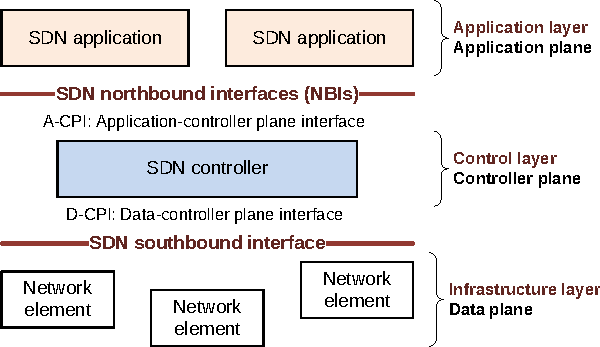
\includegraphics[width=.6\linewidth]{img/sdn_basic_schema.pdf}
    \caption{A schema of basic SDN components.}
    \label{fig:sdn-schema}
\end{figure}

\emph{Software-defined networking} is a loosely defined concept of separating the networking data plane (infrastructure layer) and the control plane (control layer) into separate components. In traditional networking architectures, each network device makes forwarding and/or routing decisions fully autonomously. SDNs separate the decision-making and data processing into distinct layers (see \cref{fig:sdn-schema}) and define two main interfaces. \emph{SDN applications} provide the \emph{SDN controller} with networking requirements using the \emph{northbound interface}. The controller then configures the actual network equipment using the \emph{southbound interface}.

\emph{OpenFlow}\footnote{\url{https://opennetworking.org/sdn-resources/openflow-switch-specification/}} is a de-facto standard protocol for the southbound interface. \emph{Container network interface (CNI)} is a specification for the northbound interface in Kubernetes and other container orchestrators.

\section{OpenFlow}

\todo{add a proper example to the table}

\emph{OpenFlow} is a protocol for configuring packet forwarders (generalized switches). The forwarding tables (see \cref{tab:openflow-forwarding-table}) in the network switches are filled with rules provided by the OpenFlow controller. The flow rules consist of two parts:

\begin{itemize}
    \item \emph{Packet matching criteria} which can include value masks for not only Ethernet header values, but also IP, transport layer protocols (TCP, UDP, ...), and more depending on the version of the OpenFlow protocol. 
    \item The action instructing the switch on what to do with the matching packets. Possible actions include dropping packets, modifying header fields, forwarding to physical or virtual ports, sending to the controller, and more.
\end{itemize}

In addition to the externally configured flow rules, the forwarding tables also contain statistics updated every time the flow rule is used. The OpenFlow controller can then query switches for these statistics.

\begin{table}[]
    \begin{center}
        \caption{Schema of an OpenFlow forwarding table}
        \label{tab:openflow-forwarding-table}
        \begin{tabular}{c|c|c}
            \textbf{Matching criteria} & \textbf{Action} & \textbf{Statistics} \\
            \hline
            \xxx{add example} & 1110.1 & a\\ % <--
            2 & 10.1 & b\\ % <--
            3 & 23.113231 & c\\ % <--
        \end{tabular}
    \end{center}
\end{table}


\section{Open vSwitch}

\emph{Open vSwitch} (OVS) is a multilayer virtual switch. OVS runs as a software switch on all major platforms and supports hardware offload for its data processing layers. The supported OpenFlow protocol allows any SDNs to use OVS in its infrastructure layer.

The internal architecture of OVS mirrors the SDN architecture (see \cref{fig:ovs-arch-schema}\todo{redraw the image or quote it properly}). \ident{ovs-vswitchd} (or just \ident{vswitchd}) is the OVS's control process. \ident{vswitchd} communicates via the OpenFlow protocol and stores the configured flow rules in a purpose-built Open vSwitch Database (OVSDB). Alternatively, the database can be accessed externally, and OVS can be configured without using the OpenFlow wire protocol.

A \emph{datapath} is the lowest component of OVS physically forwarding packets between configured ports. There are multiple datapath implementations, some of them implemented fully in the \ident{vswitchd} process, some of them using extra kernel modules for improved performance. \ident{vswitchd} translates the OpenFlow flow rules into a more efficient and simplified form. These simplified flow rules are then used by the datapaths to make forwarding decisions.

\begin{table}[h!]
    \begin{center}
        \caption{Overview of OVS components}
        \label{tab:ovs-components}
        \begin{tabular}{p{0.2\linewidth}|p{0.7\linewidth}}
            \textbf{Component} & \textbf{Description} \\
            \hline
            % FIXME this footnote might be on a wrong page :(
            \ident{ovsdb}\tablefootnote{\url{https://docs.openvswitch.org/en/latest/ref/ovsdb.7/}} & OVSDB instance storing the OpenFlow flow rules \\
            \hline
            \ident{ovs-vswitchd}\tablefootnote{\url{http://www.openvswitch.org/support/dist-docs/ovs-vswitchd.8.html}} & a process managing datapaths and providing OpenFlow configuration interface \\
            \hline
            datapath & a logical component in \ident{ovs-vswitchd}, does the actual packet forwarding \\
        \end{tabular}
    \end{center}
\end{table}


\section{Open Virtual Network}

\todo{link to documentation \url{https://access.redhat.com/documentation/en-us/red_hat_openstack_platform/13/html/networking_with_open_virtual_network/open_virtual_network_ovn}}

\emph{Open Virtual Network} (OVN) is an SDN combining Open vSwitch with network tunnels (by default GENEVE) for its infrastructure layer. Applications communicate with OVN through the \ident{northdb}, an OVSDB instance storing high-level network configuration in terms of traditional networking concepts. The \ident{ovn-northd} process translates the configuration into logical datapath flows and stores the result in the \ident{southdb} OVSDB instance. The \ident{ovn-controller} then distributes the flows from the \ident{southdb} into individual OVS databases.

\begin{table}[h!]
    \begin{center}
        \caption{Overview of OVN components}
        \label{tab:ovn-components}
        \begin{tabular}{p{0.23\linewidth}|p{0.47\linewidth}|p{0.2\linewidth}}
            \textbf{Component} & \textbf{Description} & \textbf{How it runs} \\
            \hline
            \ident{northdb} & OVSDB instance storing network configuration in terms of traditional networking concepts & centralized or distributed \\
            \hline
            \ident{ovn-northd} & process translating configuration into logical flows & centralized or distributed \\
            \hline
            \ident{southdb} & OVSDB instance storing network configuration in terms of logical flows & centralized or distributed\\
            \hline
            \ident{ovn-controller} & configures local OVS from the \ident{southdb} & locally on every node\\
        \end{tabular}
    \end{center}
\end{table}


\section{OVN-Kubernetes}

\emph{OVN-Kubernetes}\footnote{\url{https://github.com/ovn-org/ovn-kubernetes}} is a Kubernetes CNI plugin using OVN in the background. \todo{Expand with information about internal architecture.}

\section{Open vSwitch Datapath Internals}
\label{sec:ovs-packet-processing}
\todo{This whole section is not adapted to the thesis yet. It is just copy-pasted from my website.}

\begin{figure}
    \centering
    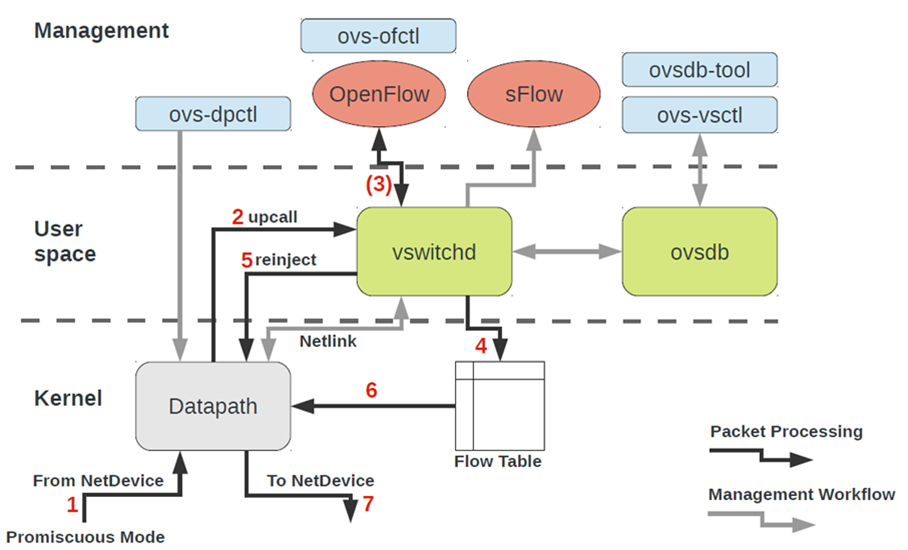
\includegraphics[width=.9\linewidth]{img/ovs_architecture_01.png}
    \caption{Schema of OVS internal architecture.}
    \label{fig:ovs-arch-schema}
\end{figure}

\ident{ovs-vswitchd} processes packets in \href{https://github.com/openvswitch/ovs/blob/e90a0727f17f6ad915a32735a8c0b282f2c8cd6f/lib/dpif.h}{datapaths}, which is essentially \href{https://github.com/openvswitch/ovs/blob/e90a0727f17f6ad915a32735a8c0b282f2c8cd6f/lib/dpif-provider.h\#L107-L117}{an interface} hiding the implementation details of low-level packet processing. The datapath does not do any decisions by itself, it's the clients of the datapath that tell it what to do by giving it simple rules to follow. In the upstream code, there are two datapath implementations - \href{https://github.com/openvswitch/ovs/blob/e90a0727f17f6ad915a32735a8c0b282f2c8cd6f/lib/dpif-netdev.c}{\ident{netdev}} and \href{https://github.com/openvswitch/ovs/blob/e90a0727f17f6ad915a32735a8c0b282f2c8cd6f/lib/dpif-netlink.c}{\ident{netlink}}.

The \ident{netdev} datapath is implemented entirely in user space, and it's multiplatform. All major operating systems are currently supported. As it's userspace only, it's less performant than the \ident{netlink} datapath and we will ignore it for the rest of this article. The \ident{netlink} datapath is Linux-specific. It resides partially in a kernel module and partially in user space. The kernel module does most of the packet processing. The userspace communicates with the kernel over a netlink socket, exchanging commands and packets. Most packets never touch the user space and are processed only in the kernel. We call this the fast-path. The alternative is the slow-path, a path through user space, which is taken every time the fast-path fails.


\subsection{Overview of the kernel and user space interactions}
\label{overview-of-the-kernel-and-user-space-interactions}

The fast-path involves matching incoming packet against a set of flow rules stored in the kernel. The rules contain actions -- instructions describing what to do next with the packet. If any of the flow rules matches, the kernel blindly executes the action. In this case, no buffering is involved, the packets are processed immediately.

The slow-path gets involved when the fast-path fails (no flow rule match) or when the action in the flow rule asks for it. In it, the packet is passed to the user-space via a netlink socket (we call this an upcall). An user-space process receives the packet, processes it according to its configuration and reinjects it back into the kernel. Additionally, a new flow rule can be installed into the kernel to speed up future processing of similar packets. The slow-path buffers packets when they are passed from kernel to user-space.

\subsection{The fast-path}
\label{the-fast-path}

\subsubsection{The data structures}
\label{the-data-structures}

The flow table (\href{https://elixir.bootlin.com/linux/v6.2.6/source/net/openvswitch/flow_table.h\#L62}{\ident{struct\ flow\_table}}) is an in-kernel data structure, which stores flows rules (\href{https://elixir.bootlin.com/linux/v6.2.6/source/net/openvswitch/flow.h\#L221}{\ident{struct\ sw\_flow}}) and allows for fast matching with individual packets. Every flow also contains a list of actions (\href{https://elixir.bootlin.com/linux/v6.2.6/source/net/openvswitch/flow.h\#L206}{\ident{struct\ sw\_flow\_actions}}).

Every flow has a flow key (\href{https://elixir.bootlin.com/linux/v6.2.6/source/net/openvswitch/flow.h\#L75}{\ident{struct\ sw\_flow\_key}}) and a bitmask (\href{https://elixir.bootlin.com/linux/v6.2.6/source/net/openvswitch/flow.h\#L183}{\ident{struct\ sw\_flow\_mask}}). The combination of both of these enables the packet matching. The key is a complex structure with parsed out packet header values. It can be created from any Ethernet frame (\href{https://elixir.bootlin.com/linux/v6.2.6/source/net/openvswitch/flow.c\#L886}{\ident{key\_extract}}). The mask then tells us which bits between the extracted packet key and the flow key must match.


\subsubsection{The matching algorithm}
\label{the-matching-algorithm}

When processing a packet, we create the corresponding flow key and look for matching flows in the flow table. The packet can match any number of flows, but we always use the first one we find. The userspace component is made responsible for preventing overlapping conflicting flow rules.

The flow table stores the flow in a hash table, where the key is the masked \ident{sw\_flow\_key}. Therefore, to find a flow for a packet, we must try several masks. The lookup procedure could look like this:

\begin{verbatim}
    def lookup(flow_table, key):
        for mask in flow_table.mask_array:
            masked_key = apply mask to key
            if masked_key in flow_table.flows:
                return flow_table.flows[masked_key]
        return None
\end{verbatim}
    

The real implementation (\href{https://elixir.bootlin.com/linux/v6.2.5/source/net/openvswitch/flow_table.c\#L785}{\ident{ovs\_flow\_tbl\_lookup\_stats}}) is in principle similar, but more optimized:

\begin{enumerate}
\def\labelenumi{\arabic{enumi}.}
\item
  The kernel keeps mask usage statistics and the \ident{mask\_array} is
  kept sorted with the most used masks first
  (\href{https://elixir.bootlin.com/linux/v6.2.5/source/net/openvswitch/flow_table.c\#L1107}{\ident{ovs\_flow\_masks\_rebalance}}).
  This happens
  \href{https://elixir.bootlin.com/linux/v6.2.5/source/net/openvswitch/datapath.c\#L2536}{periodically}
  based on a time interval.
\item
  There is already a \ident{sk\_buff}
  \href{https://elixir.bootlin.com/linux/v6.2.5/source/include/linux/skbuff.h\#L1537}{hash}
  based on source/destination addresses and ports. The lookup procedure
  makes use of the hash by having a fixed size
  (\href{https://elixir.bootlin.com/linux/v6.2.5/source/net/openvswitch/flow_table.c\#L41}{256})
  hash table storing references to their masks. The cached masks are
  then tried first. If there is no match, standard lookup over all masks
  follows. This helps with burst performance.
\end{enumerate}

\subsection{The slow-path}
\label{the-slow-path}

The user space process (\href{https://www.man7.org/linux/man-pages/man8/ovs-vswitchd.8.html}{\ident{ovs-vswitchd}}) communicates with the kernel over netlink socket. When packet leaves the
fast-path, it is temporarily buffered in a queue (\href{https://elixir.bootlin.com/linux/v6.2.6/source/net/openvswitch/datapath.c\#L311}{\ident{ovs\_dp\_upcall}}) when crossing the kernel boundary.

\ident{ovs-vswitchd} reads packets from the kernel in several threads. The datapath interface defines a \href{https://github.com/openvswitch/ovs/blob/e90a0727f17f6ad915a32735a8c0b282f2c8cd6f/lib/dpif-provider.h\#L387-L408}{\ident{recv}} function for receiving a single packet from the kernel. The netlink datapath implements it with the function \href{https://github.com/openvswitch/ovs/blob/e90a0727f17f6ad915a32735a8c0b282f2c8cd6f/lib/dpif-netlink.c\#L3132-L3134}{\ident{dpif\_netlink\_recv}}.

Higher up, the \ident{recv} datapath interface function is used in generic \href{https://github.com/openvswitch/ovs/blob/e90a0727f17f6ad915a32735a8c0b282f2c8cd6f/lib/dpif.c\#L1591-L1611}{\ident{dpif\_recv}} which also provides an useful tracepoint \href{https://github.com/openvswitch/ovs/blob/e90a0727f17f6ad915a32735a8c0b282f2c8cd6f/lib/dpif.c\#L1618}{\ident{dpif\_recv\_\_recv\_upcall}} for measurements. Even higher up the abstraction stack, the function \href{https://github.com/openvswitch/ovs/blob/e90a0727f17f6ad915a32735a8c0b282f2c8cd6f/ofproto/ofproto-dpif-upcall.c\#L829-L830}{\ident{recv\_upcalls}} in the file \ident{ofproto-dpif-upcall.c} reads packets in batches, which are then processed by \href{https://github.com/openvswitch/ovs/blob/e90a0727f17f6ad915a32735a8c0b282f2c8cd6f/ofproto/ofproto-dpif-upcall.c\#L1639-L1641}{\ident{handle\_upcalls}}. The \ident{handle\_upcalls} function essentially transforms the list of packets into a list of operations that should be executed on the datapath. This includes adding new flows to the datapath as well as simply sending packets where they belong.

Parallel with upcall processing, OVS also runs several maintenance tasks. A \href{https://github.com/openvswitch/ovs/blob/e90a0727f17f6ad915a32735a8c0b282f2c8cd6f/ofproto/ofproto-dpif-upcall.c\#L3312-L3336}{balancing task} makes sure, that when the system is under stress, the most used flow rules are in the kernel. \href{https://github.com/openvswitch/ovs/blob/e90a0727f17f6ad915a32735a8c0b282f2c8cd6f/ofproto/ofproto-dpif-upcall.c\#L83-L111}{A revalidator task} periodically reads statistics from the kernel and most importantly, removes old unused flows.

% TODO add sources
%
% \begin{center}\rule{0.5\linewidth}{0.5pt}\end{center}
% 
% \hypertarget{sources}{%
% \section{Sources}\label{sources}}
% 
% \begin{itemize}
% \tightlist
% \item
%   \href{https://docs.openvswitch.org/en/latest/contents/}{Open vSwitch
%   online documentation}
% 
%   \begin{itemize}
%   \tightlist
%   \item
%     \href{https://docs.openvswitch.org/en/latest/topics/datapath/}{Open
%     vSwitch Datapath Development Guide}
%   \end{itemize}
% \item
%   \href{https://elixir.bootlin.com/linux/v6.2.6/source}{Linux Kernel
%   source code}
% \item
%   \href{https://github.com/openvswitch/ovs/tree/51778134d4c8a84801230b1e5a7d59e180d9e8b5}{Open
%   vSwitch source code}
% \item
%   \href{https://developers.redhat.com/articles/2022/02/07/investigating-cost-open-vswitch-upcalls-linux}{RedHat
%   Developer Blog: Investigating the cost of Open vSwitch upcalls in
%   Linux}
% \item
%   \href{https://hustcat.github.io/an-introduction-to-ovs-architecture/}{An
%   introduction to OVS architecture}
% \end{itemize}
\chapter{Experimental environment}
\label{chap:env}

This chapter describes the environment we used for running our experiments. The information provided here should allow anyone to replicate our measurements.

\section{Hardware}
\label{sec:hw-env}

For our research, we used two experimental cluster with different hardware configurations. One installation run virtualized on Proxmox VE with only a single physical host. The other installation used dedicated hardware. When we write about an experiment and do not specify where it runs, we are presenting results from the cluster on dedicated hardware. However, most of the measurements can be replicated in a virtualized environment without a significant impact on the outcome.

\paragraph{Virtualized installation}
We used the virtualized environment for development and debugging. The physical host was running Proxmox VE 7.4-3, and it was configured with an Intel\textsuperscript{\textregistered} Core\textsuperscript{TM} i7-3770 CPU running at 3.40 GHz with $4$ cores, $8$ threads, and $31.23$ GiB of RAM.

The virtual machines used for the cluster nodes were each configured with $4$ virtual cores and $4$ GiB of RAM. We had initially started experimenting with $2$ CPU cores per node to prevent overprovisioning, but our workloads always fully stressed only one node (always \kb{2}), and we were mostly interested in system behavior with multiple threads. The overprovisioning did not seem to cause any problems.

The cluster nodes were equipped with $2$ virtual network interfaces connected to two virtual Linux bridges on the host. We used one interface for system management and WAN access. Tthe other bridge was used for cluster interconnect. We did not artificially limit the throughput or latency of the link between nodes. When measured between \kb{2} and \kb{3} using \ident{iperf3} with the default configuration and \ident{ping} with $100$ samples, the throughput was $14.5$ Gbps and the average round trip time $0.383$ ms.

\paragraph{Dedicated hardware}

We used the cluster with dedicated hardware to validate the results observed in the virtual environment. The nodes were Dell PowerEdge R730 servers, configured with Intel\textsuperscript{\textregistered} Xeon\textsuperscript{\textregistered} CPU E5-2690 v4 running at 2.60GHz with $14$ cores, $28$ threads, and $131$ GB of RAM.

Similar to the virtualized nodes, the dedicated nodes had 2 network interfaces. One management 1 GbE interface was connected to the Internet, and another cluster only 10 GbE interface was connected to a switch. We configured the switch to use VLANs to isolate the cluster traffic from all other ports. While we did not have the opportunity to use a fully dedicated switch, the switch should have had enough capacity that it would not be a bottleneck. The average round trip time between \kb{2} and \kb{3} (\ident{ping -c 100}) was $0.104$ ms.

\section{Software environment}
\label{sec:sw-env}

We run our experiments and measurements on a Kubernetes cluster with OVN-Kubernetes as the CNI plugin and Docker as the container runtime. OVN-Kubernetes was installed using containerized setup following the official installation guide \cite{OVNInstallGuide}. We used Fedora 38 as the base Linux distribution. To allow reproducibility, we fully automated the installation procedure. Installation scripts with usage instructions can be found in \cref{chap:install}.

In our experiments, we always used a three-node cluster with one node dedicated as a control node. We didn't test cluster installations configured for high availability (HA). We focused on the internals of OVS, a part of low-level networking infrastructure. We do not expect any significant difference between HA and non-HA clusters.

We named our cluster nodes \kb{1}, \kb{2}, and \kb{3}. The node \kb{1} is always the control node, our experiments always run on \kb{2}.

\subsection{OVN-Kubernetes configuration}
\label{subsec:ovnkube-limits}

We deployed a fully containerized OVN-Kubernetes, meaning that even OVS was deployed in a privileged container. The default OVS container spec file contains \href{https://github.com/ovn-org/ovn-kubernetes/blob/master/dist/templates/ovs-node.yaml.j2\#L84-L90}{this resource limit}:

\begin{verbatim}
resources:
    requests:
        cpu: 100m
        memory: 300Mi
    limits:
        cpu: 200m
        memory: 400Mi
\end{verbatim}

We have manually removed this limit for most of our experiments. We have also tested with the limit active and we always explicitly mention it when it is the case.

\subsection{OVS modifications}

Instead of the default OVS container, we configured our systems with a modified version to improve observability. Our changes included:

\begin{itemize}
    \item We added development tools (e.g. \ident{gdb}, \ident{perf}, ...) to the container image.
    \item We recompiled \ident{ovs-vswitchd} to include additional user statically-defined tracing (USDT) \cite{USDT} probes
    \item We included debug symbols in the \ident{ovs-vswitchd} executable
\end{itemize}

Implementation details and instructions on how to replicate our build are in \cref{chap:ovs-mod}.

\subsection{Kubernetes configuration}

We always deployed three different pods to the Kubernetes cluster. The spec files are attached to this work. The pods were:

\begin{itemize}
    \item \ident{arch} on \kb{2} -- a pod running the latest Arch Linux Docker image. We used this pod for the main part of our experiments.

    \item \ident{victim} on \kb{2} -- again, a pod with the latest Arch Linux image. We used it to measure the impact of our experiments on pods sharing the same node.

    \item \ident{reflector} on \kb{3} -- a privileged Arch Linux container with a custom raw-socket-based packet reflector and \ident{iptables} rule preventing the kernel from sending ICMP connection refused packets. The reflector swapped the Ethernet and IP addresses in the received packets and sent them out again.
\end{itemize}

\subsection{Experiment implementation}

We developed our experiments mainly in Rust. Everything is contained within one project in a tool we call the \ident{analyzer}. In the few cases when Rust was not the best language for the task, we embedded scripts in other languages (mainly Bash and Python) in the Rust executable itself. Our Rust code always provides an entry point.

The main reasoning behind the language and architecture choice was personal preferences and ease of distribution -- the ability to create a single statically-linked executable that would work almost anywhere.

Implementation details and usage instructions are in \cref{chap:analyzer}.

\subsection{Clock synchronization}

All our experiments use Linux's \ident{CLOCK\_MONOTONIC} clock for timekeeping. Because we measure everything on a single node, \kb{2}, the clock is perfectly consistent across different containers. There could be small discrepancies due to synchronization between CPU cores and scheduling, but we are mostly concerned about larger time scales so we assume these discrepancies will not affect our results.


\chapter{Experiment design}
\label{chap:design}

As we showed in \cref{chap:refs}, OVS inserts flow rules into datapaths on demand after upcalls. Therefore, some packets require much more processing and can slow the system down. Eelco Chaudron investigated the cost of an upcall in OVS\todo{link source} using eBPF probes in the Linux kernel. His experiments show that processing a packet through the slow path can take anywhere between \qty{700}{\us} and \qty{10}{\ms} extra compared to the fast path.

Based on this knowledge, we tried to answer the following questions about OVS internals:

\begin{itemize}
    \item When are flow rules removed from the datapaths? (\cref{design:flow-eviction})
    \item What is the cost of an upcall when measured from the user space? (\cref{design:upcall-cost})
    \item Which packets generate upcalls? (\cref{design:upcall-generators})
    \item What is the impact of artificial upcall-only traffic on the performance of the whole system? (\cref{design:upcall-impact})
\end{itemize}

The following sections describe our methods to answer the questions. The next chapter discusses our results.


% quote https://developers.redhat.com/articles/2022/02/07/investigating-cost-open-vswitch-upcalls-linux


\section{Removal of flow rules from datapaths}
\label{design:flow-eviction}

We can observe an effect of an upcall using the \ident{ping} tool. The first packet has higher latency than the rest of the ICMP packets.

\vspace{0.5cm}

\begin{lstlisting}[caption=Output of the \ident{ping} command in the virtualized environment, captionpos=b, basicstyle=\ttfamily\scriptsize]
[root@kb2 ~]# ping -c 5 kb3
PING kb3 (192.168.1.223) 56(84) bytes of data.
64 bytes from kb3 (192.168.1.223): icmp_seq=1 ttl=64 time=1.19 ms
64 bytes from kb3 (192.168.1.223): icmp_seq=2 ttl=64 time=0.404 ms
64 bytes from kb3 (192.168.1.223): icmp_seq=3 ttl=64 time=0.365 ms
64 bytes from kb3 (192.168.1.223): icmp_seq=4 ttl=64 time=0.424 ms
64 bytes from kb3 (192.168.1.223): icmp_seq=5 ttl=64 time=0.304 ms

--- kb3 ping statistics ---
5 packets transmitted, 5 received, 0% packet loss, time 4062ms
rtt min/avg/max/mdev = 0.304/0.536/1.185/0.326 ms
\end{lstlisting}

The first packet delay is absent when we run the \ident{ping} command for the second time shortly after the first. The higher latency is visible again. This behavior can be explained by a flow rule eviction timeout that removes the rule from the datapath's forwarding table.

Assuming the timeout stays constant, we can measure it by varying the interval between ICMP packets. The dependency between the measured latency and the time delay should be constant except for one sharp increase in latency when the delays get longer than the timeout.

\paragraph{Our experiment}
We conducted the experiment in the following way:

\begin{enumerate}
    \item Generate a random number $D$ in the interval $\interval{8}{12}$
    \item sleep for $D$ seconds
    \item run \ident{ping -c 2 192.168.1.221}
    \item log $D$ and both round trip times
    \item goto step 1 until we have enough
\end{enumerate}

We chose the interval based on non-rigorous preliminary experiments. After plotting RTT's dependence on the delay $D$, we expect to see:

\begin{itemize}
    \item The first RTT data points will form a line with a sharp increase at a value of $D$ corresponding to the eviction timeout

    \item The second RTT data points will form only a single horizontal line.
\end{itemize}

Results of this experiment can be found in \cref{res:eviction-timeout}.

\section{Cost of an upcall}
\label{design:upcall-cost}

Eelco Chaudron's research into the cost of an upcall used eBPF to measure upcall cost directly in the kernel. However, as we saw in the previous section, upcalls have visible effects outside of the kernel.

The unchanged experiment devised in the previous section provides us with a direct measurement of the observable upcall effect. In each data point, we can subtract the two round-trip-times to get an insight into how much time upcall costs.

While this measurement methodology leads to less precise results than when directly measuring the in-kernel execution time using eBPF, we can use it to measure the upcall cost without special privileges on publicly deployed cloud hosting services.\todo{má smysl tohle zmiňovat, když to nezkusím? Napsal jsem do MetaCentra a domluvili jsme se, ze se mi ozvou. Ale zatim nic.}

Our results can be found in \cref{res:upcall-cost}.

\section{Packets generating upcalls}
\label{design:upcall-generators}

To stress-test the slow path, we have to be able to generate upcalls consistently. We have to find types of packets that will repeatedly miss all installed flow rules in the OVS datapath. We have a choice between a static analysis and a dynamic analysis of OVS.

We chose to approach the problem using dynamic analysis. We decided on dynamic analysis instead of static analysis because the results depend on OVS, the whole SDN, and its configuration. For static analysis, the search space is just too large. Also, the dynamic analysis tooling can be later reused on different OVS deployment than ours.

Our experiment sends varying packets in batches based on their type and monitors the upcalls and flow table changes using kprobes in the kernel and user statically-defined tracing (USDT) probes in \ident{ovs-vswitchd}.

The flow rules in OVS datapaths use the \ident{struct sw\_flow\_key}\todo{link} to represent the flow key. For every field of that structure, our measurement tool sends 1000 packets with the corresponding packet header field randomized and everything else fixed at arbitrary values.

We used Scapy to generate the packets. For example, the code to generate random TTL values in an IPv4 packet looks like this:

\begin{verbatim}
tag("IP(ttl)")
sendp(Ether(dst="aa:bb:cc:dd:ee:ff") / IP(dst="10.244.1.1", ttl=RandByte()), count=1000)
sleep(11)  # more than the eviction timeout
\end{verbatim}

Because we used dynamic analysis, we can not be certain that we covered all possible cases. We can draw some general conclusions from the measurement results and look into the source code for additional insights. However, there is always the possibility that we missed something.

\section{Impact of upcall-only traffic}
\label{design:upcall-impact}

\paragraph{Stress testing tool}
From the previous experiment, we learned that randomized unicast Ethernet source addresses generate upcalls. We used this knowledge to write a custom tool for sending minimalistic Ethernet frames. The Ethernet header needs only 14 bytes, but we used 16-byte packets due to slightly better performance. Instead of randomization, we filled the source Ethernet addresses with an increasing integer sequence.

Our tool is optimized for controlled and regular packet generation. Configured with a time interval between packets or a desired packet frequency, it tries to send packets as regularly as possible:

\begin{verbatim}
start_time = clock()
sent = 0
while True:
    now = clock()
    while we should have sent more packets than we sent:
        sent a new packet
        sent += 1
    
    sleep( until next packet is scheduled )
\end{verbatim}

Only instead of sending the packets one by one every time, we send them in batches using \ident{io\_uring} if it is possible. When we set the interval to \qty{1}{\ns} (zero is not possible due to division by zero), we can reach roughly 210k packets per second in a single thread on the dedicated test server.

\paragraph{The experiment}
For our experiment, we stressed OVS using our tool and monitored the system. We mainly measured OVS's memory consumption, the load average of the whole system and latencies observable from the \ident{victim} pod.

The results of the experiment can be found in \cref{res:upcall-stress}.
%\chapter{Results of the experiments}
\label{chap:exp}

\section{Flow eviction timeout}
\label{res:eviction-timeout}

\begin{figure}
    \centering
    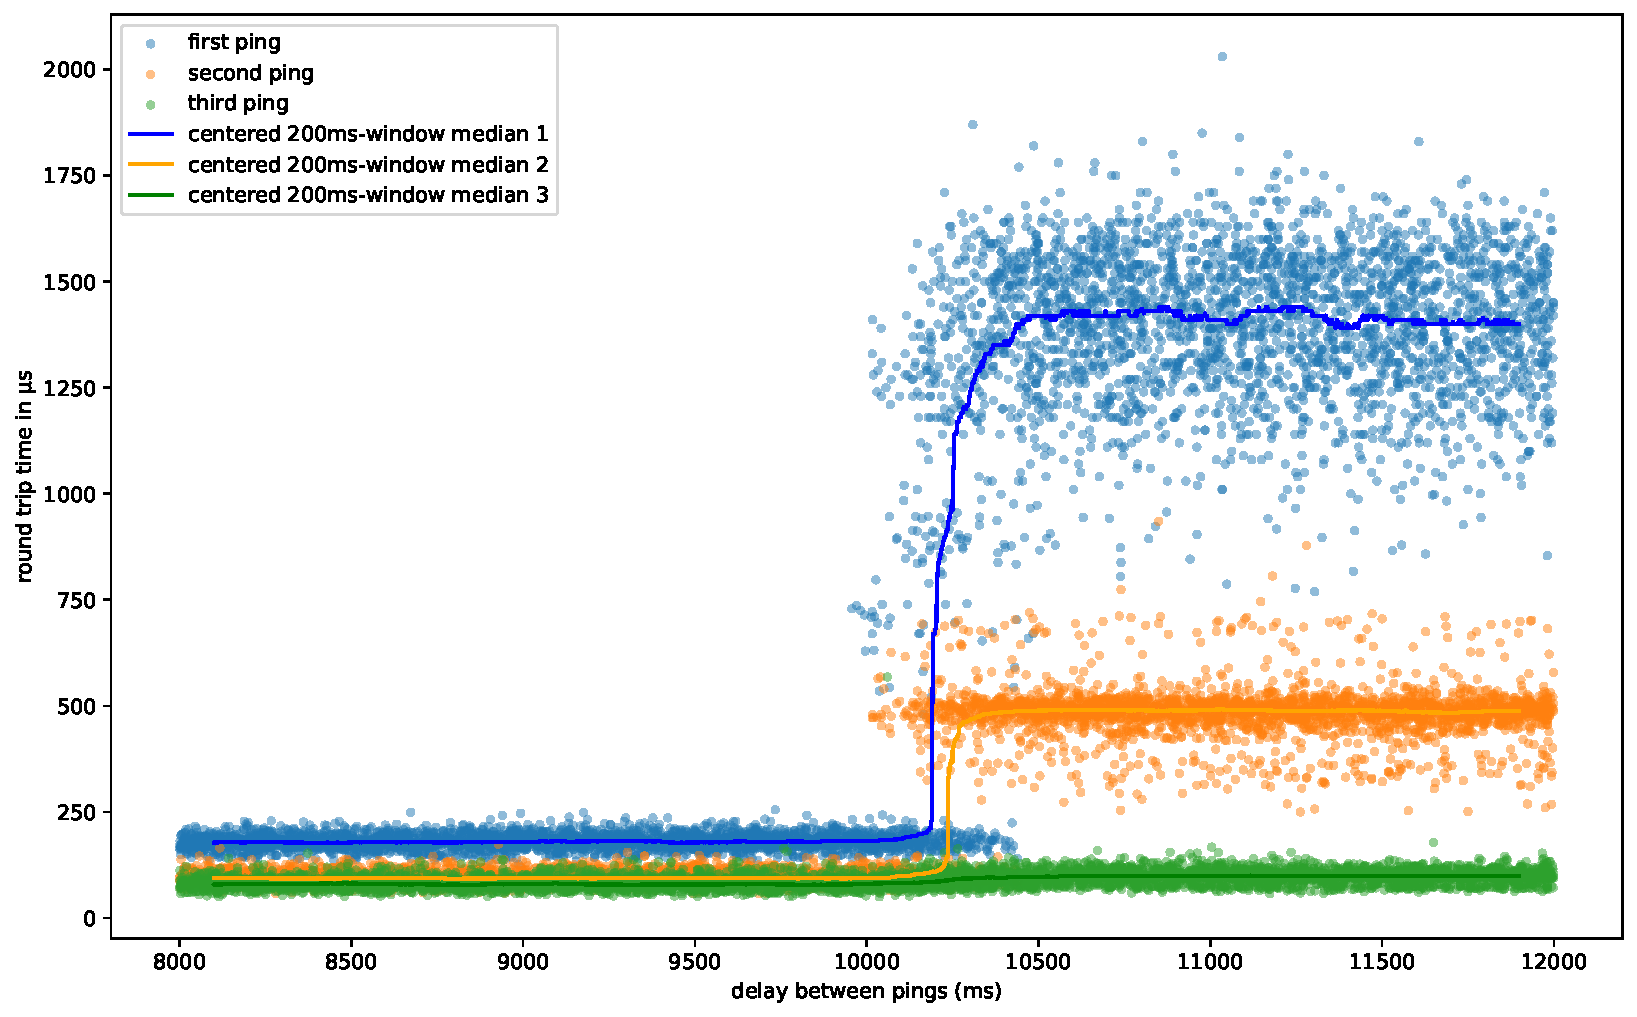
\includegraphics[width=.9\linewidth]{img/randomized_eviction_timeout.pdf}
    \caption{Results of the eviction timeout experiment}
    \label{fig:plot-eviction-timeout}
\end{figure}

\paragraph{The eviction timeout} The measured latencies of the experiment (\cref{fig:plot-eviction-timeout}) show the flow rule eviction taking effect about $10$ seconds after the last datapath rule installation. The observed value is not exact, but it is probably reasonable to assume the developers chose a nice-looking number. We hypothesize that the noise in the location of the increase is introduced mainly by infrequent eviction checks.

Following these experimental findings, we searched the source code and it specifies exactly $10$ seconds as the default eviction timeout. The experimental findings are consistent with the source code. The default rule timeout defined in the file \ident{ofproto/ofproto.h}:
\begin{verbatim}
#define OFPROTO_MAX_IDLE_DEFAULT 10000 /* ms */
\end{verbatim}

The file \ident{ofproto/ofproto-dpif-upcall.c} contains the code enforcing the timeout in the function \ident{revalidate()}:

\begin{verbatim}
if (kill_them_all || (used && used < now - max_idle)) {
    result = UKEY_DELETE;
}
\end{verbatim}

The eviction is handled by the revalidator threads, which run periodically roughly every 500ms. This confirms our hypothesis about the roughly 500ms spread of the observable timeout effect.

\begin{verbatim}
// in file ofproto/ofproto.h:321
#define OFPROTO_MAX_REVALIDATOR_DEFAULT 500 /* ms */

// in the ofproto/ofproto_dpif_upcall.c:1052
// in function udpif_revalidator()
poll_timer_wait_until(start_time + MIN(ofproto_max_idle,
                                    ofproto_max_revalidator));
\end{verbatim}

\paragraph{Difference in latency below timeout}
\Cref{fig:plot-eviction-timeout} shows a difference between round trip times for the first and second packet even below the eviction timeout. The difference is small, so we assume that this can be caused by CPU caches. We did not investigate this further.

\paragraph{Increase in round trip time of the second ping}
\Cref{fig:plot-eviction-timeout} also shows an increased latency for the second ping after the eviction timeout. We hypothesize that it could be caused by the fixed size flow lookup cache described in \cref{subsec:matching-algo}. The upcall installs the new flow, but the lookup cache is filled only after the first use (i.e. the second packet of the flow, the second ICMP ping). In other words, if we had three packets, their journey through the \ident{openvswitch} module would be as follows:

\begin{enumerate}
    \item A cache miss, followed by a flow table miss. Leads to an upcall and a new flow rule.
    \item A cache miss, which requires a full flow table scan. The cache is filled.
    \item Cache hit.
    \item All consecutive packets hit the cache unless the cache entry is somehow overwritten.
\end{enumerate}

The third RTT measurement behaves as expected by our hypothesis. We shortly experimented with even more consecutive measurements and they were all the same.


\section{Cost of an upcall}
\label{res:upcall-cost}

\paragraph{Upcall processing cost}
As discussed in \cref{chap:design}, the round trip time increase can be attributed to the cost of upcall processing. In the previous section, we noticed an increased latency with the second RTT measurement, possibly a cache miss in the kernel datapath.  We can estimate the cost of an upcall using this data. We calculated the difference between the first and the second ping measurements and assume the result is the lower bound for the upcall cost. Either our hypothesis about the cache miss is correct. Then the difference would be exactly the time spent processing the upcall. Or, we are wrong and the higher second ping latencies are caused by some additional factor which is not normally present. In that case, the upcall cost would be certainly equal to or higher than our result. We used only the data points with above $10.5$ second delay since the last measurement.

% QT_QPA_PLATFORM=xcb python postprocessing/randomized_eviction_timeout.py results/randomized_eviction_timeout/*.csv
\begin{table}[h!]
    \begin{center}
        \caption{Statistics of measured round trip times when the interval > 10.5 seconds}
        \label{tab:upcall-cost}
        \begin{tabular}{r|S[table-format=4.2]S[table-format=4.2]S[table-format=4.2]}
            & \textbf{First ping RTT} & \textbf{Second ping RTT} & \textbf{Difference} \\
            \hline
            \textbf{\#samples} & 1596 & 1596 & 1596 \\
            \textbf{Mean} & 1399.94 & 483.66 & 916.28 \\
            \textbf{Std} & 162.74 & 59.73 & 154.52\\
            \hline
            \textbf{Min} & 769 & 250 & 149 \\
            \textbf{25th percentile} & 1300 & 467 & 814 \\
            \textbf{Median} & 1410 & 488.0 & 935 \\
            \textbf{75th percentile} & 1520 & 504 & 1031 \\
            \textbf{Max} & 2030 & 878 & 1460 \\
        \end{tabular}
    \end{center}
\end{table}

The mean of the latency difference is within $916.28 \pm 7.59$ \si{\micro\second} with 95\% confidence. 

\paragraph{Comparison to previous results}

We can not directly compare our results with \href{https://developers.redhat.com/articles/2022/02/07/investigating-cost-open-vswitch-upcalls-linux}{Eelco Chaudron's}, because we do not have the same test environment. Under simulated normal conditions, he concluded that the time from the kernel's upcall invocation til the kernel's packet execution is on average $149.83$ \si{\micro\second} ($56446$ samples). Our results are 6x higher. In the same article, he notes:

\begin{quote}
My sample runs have shown what I want to emphasize in this article: The way the upcalls are generated highly influences the outcome of the upcall costs.
\end{quote}

And he shows, that under stress the average upcall cost can be $29367.91$ \si{\micro\second} ($13807$ samples). Therefore, all we can say is that our results are in the range of possible upcalls costs according to his article.

%┌────────────┬───────────────────────────┬─────────────┬─────────────┬───┬─────────────┬──────────────┬──────────────┬─────────────┐
%│ describe   ┆ us_since_last_measurement ┆ us_latency1 ┆ us_latency2 ┆ … ┆ us_latency5 ┆ first_second ┆ second_third ┆ first_third │
%│ ---        ┆ ---                       ┆ ---         ┆ ---         ┆   ┆ ---         ┆ ---          ┆ ---          ┆ ---         │
%│ str        ┆ f64                       ┆ f64         ┆ f64         ┆   ┆ f64         ┆ f64          ┆ f64          ┆ f64         │
%╞════════════╪═══════════════════════════╪═════════════╪═════════════╪═══╪═════════════╪══════════════╪══════════════╪═════════════╡
%│ count      ┆ 1596.0                    ┆ 1596.0      ┆ 1596.0      ┆ … ┆ 1596.0      ┆ 1596.0       ┆ 1596.0       ┆ 1596.0      │
%│ null_count ┆ 0.0                       ┆ 0.0         ┆ 0.0         ┆ … ┆ 0.0         ┆ 0.0          ┆ 0.0          ┆ 0.0         │
%│ mean       ┆ 1.1492e7                  ┆ 1399.93985  ┆ 483.663534  ┆ … ┆ 78.058271   ┆ 916.276316   ┆ 385.445489   ┆ 1301.721805 │
%│ std        ┆ 291241.87679              ┆ 162.744156  ┆ 59.725571   ┆ … ┆ 14.354351   ┆ 154.522521   ┆ 59.936718    ┆ 162.502307  │
%│ min        ┆ 1.1001e7                  ┆ 769.0       ┆ 250.0       ┆ … ┆ 48.0        ┆ 149.0        ┆ 131.0        ┆ 672.0       │
%│ max        ┆ 1.1999e7                  ┆ 2030.0      ┆ 878.0       ┆ … ┆ 168.0       ┆ 1460.0       ┆ 785.0        ┆ 1945.0      │
%│ median     ┆ 1.1498e7                  ┆ 1410.0      ┆ 488.0       ┆ … ┆ 75.0        ┆ 935.0        ┆ 390.0        ┆ 1313.0      │
%│ 25%        ┆ 1.1237e7                  ┆ 1300.0      ┆ 467.0       ┆ … ┆ 69.0        ┆ 814.0        ┆ 365.0        ┆ 1197.0      │
%│ 75%        ┆ 1.1749e7                  ┆ 1520.0      ┆ 504.0       ┆ … ┆ 85.0        ┆ 1031.0       ┆ 408.0        ┆ 1426.0      │
%


\section{Packets generating upcalls}
\label{res:upcall-generators}
\todo{graf je netisknutelny a neumim ho ani zmensit, co se s tim da udelat?}

\begin{figure}
    \centering
    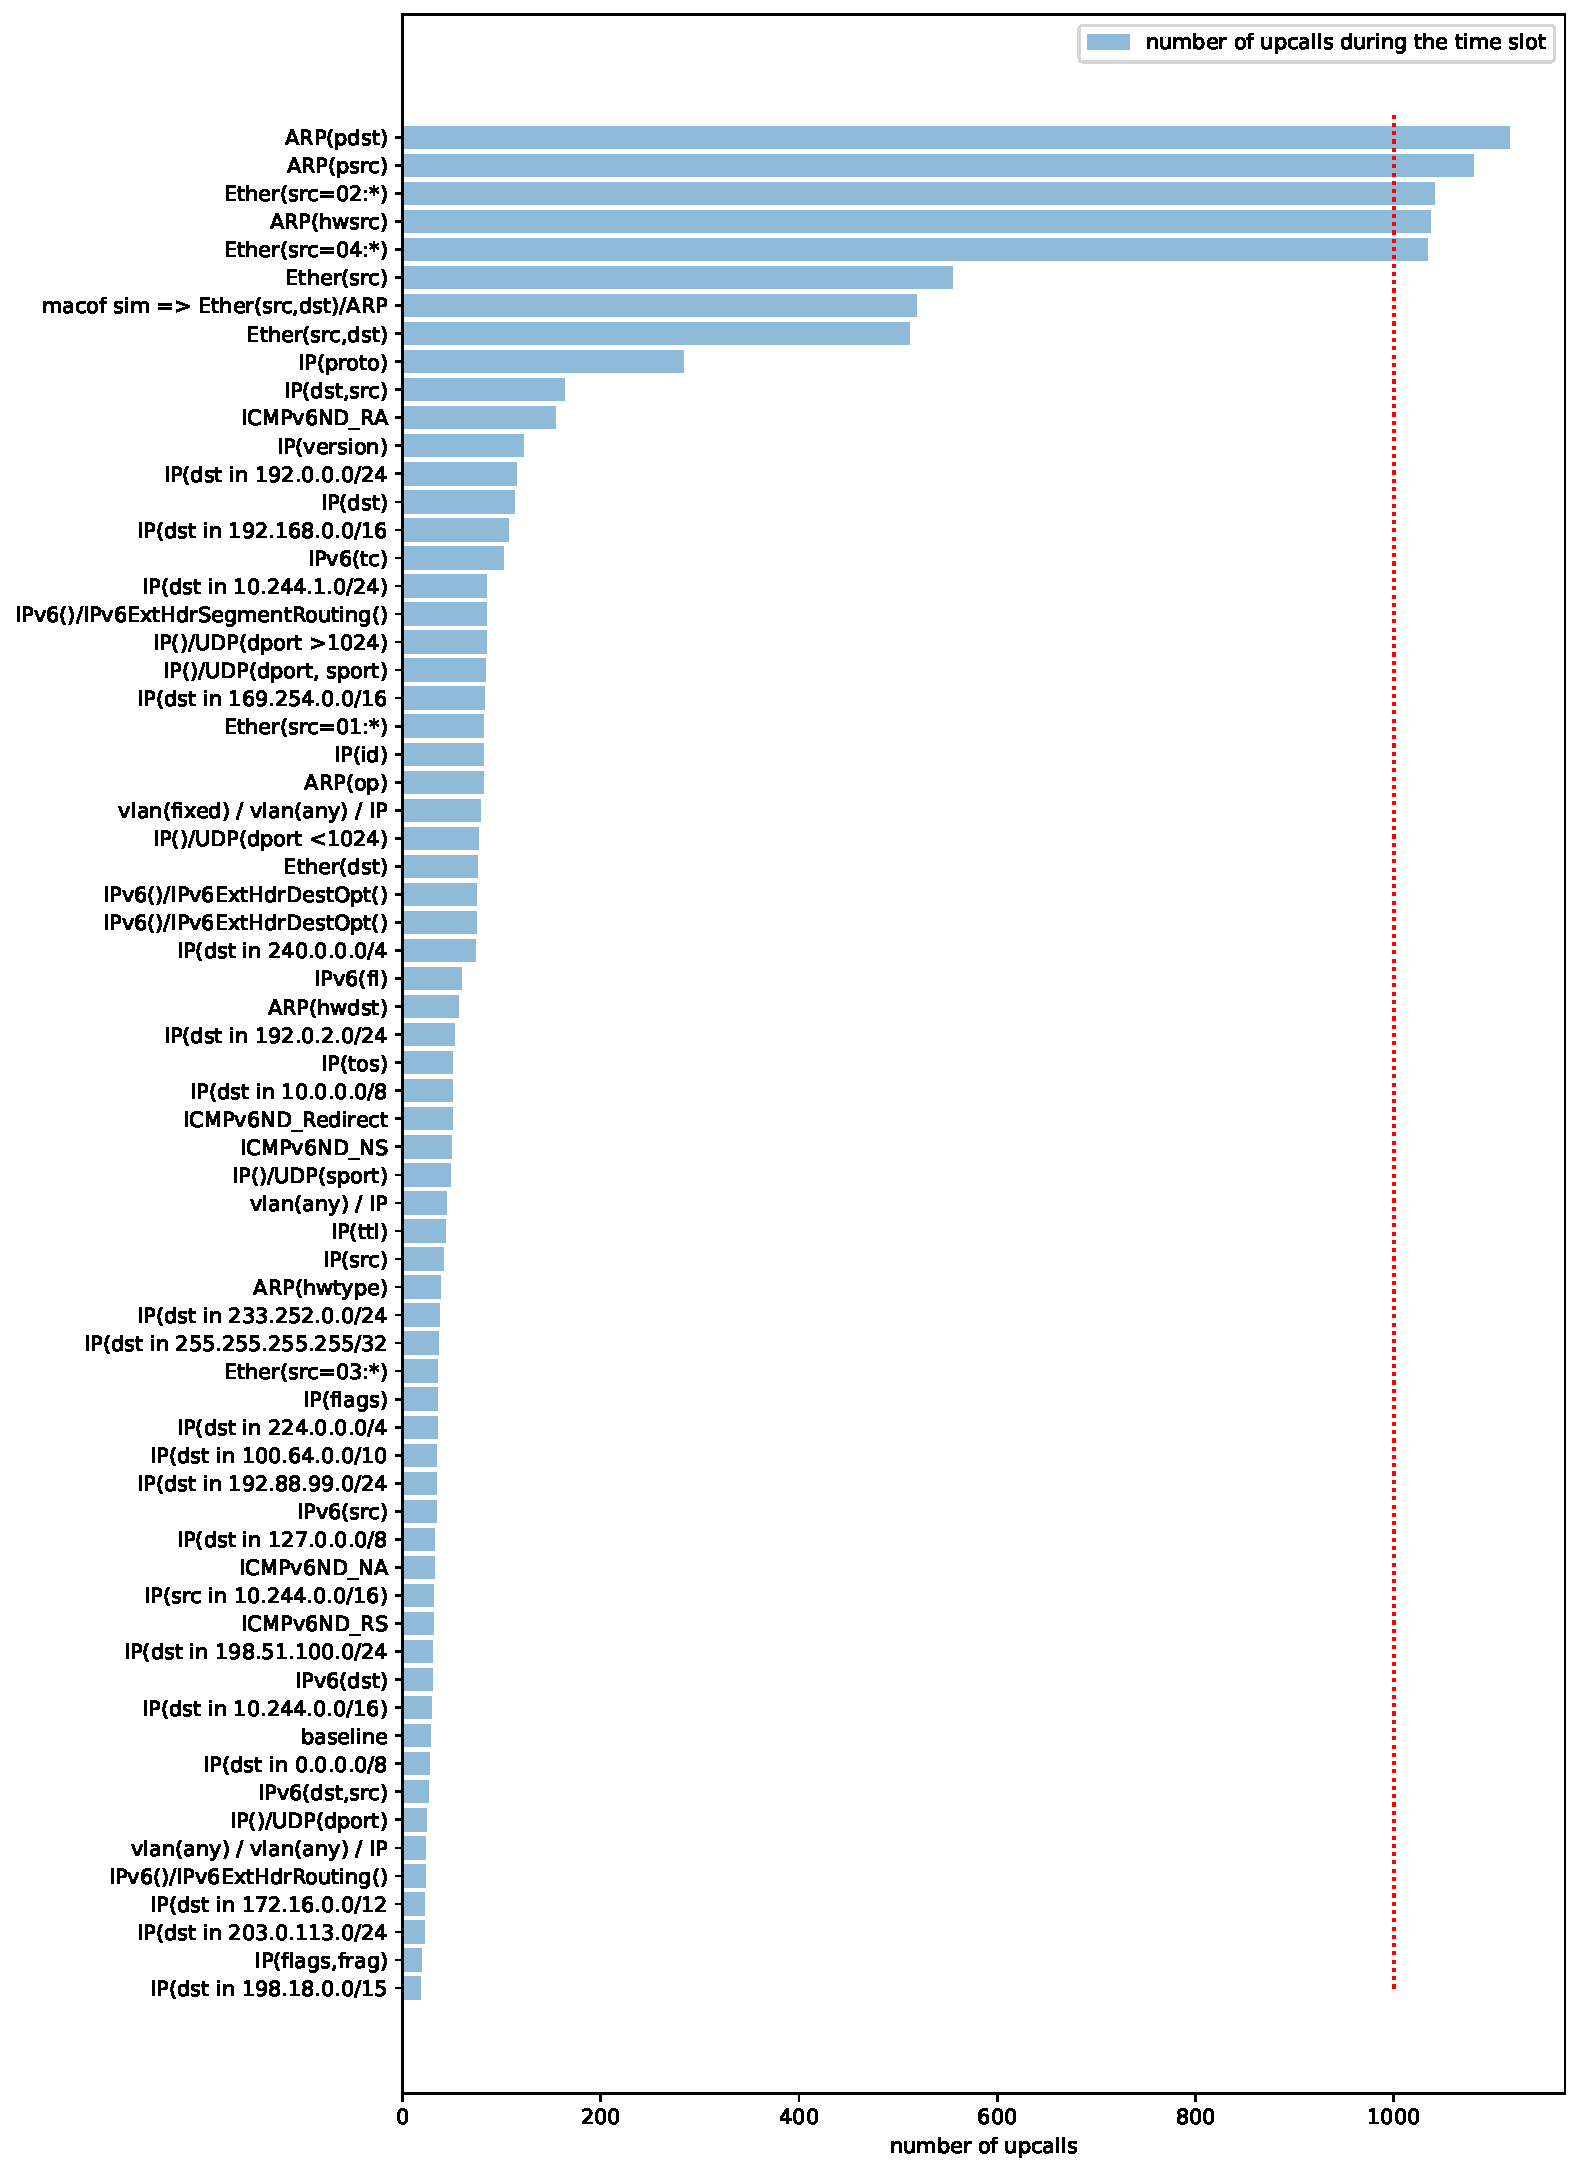
\includegraphics[width=\linewidth]{img/packet_fuzz.pdf}
    \caption{Number of upcalls generated by varying certain header fields in packets}
    \label{fig:plot-packet-fuzz}
\end{figure}

\Cref{fig:plot-packet-fuzz} shows the number of upcalls generated after sending 1000 crafted packets differing only in a value of a specified header field. We are interested in the peak of the plot, they signify packet types that consistently generate upcalls. The most significant being varying Ethernet source addresses and address fields in ARP packets.

\subsection{Ethernet source addresses}
\label{subsec:ethernet}

Varying the Ethernet source address in the unicast range (the least significant bit of the first byte has to be 1) generates new upcalls. The flow rules being inserted into the flow table are similar to the following example\footnote{dumped with \ident{ovs-dpctl dump-flows}}:

\begin{verbatim}
recirc_id(0),in_port(9),
    eth(src=04:6a:68:88:2b:eb),eth_type(0x0800),ipv4(frag=no),
    packets:0, bytes:0, used:never, actions:drop
\end{verbatim}

OVN has a feature called port security which can be enabled for logical switch ports. By enabling port security on a port, MAC spoofing is prevented and all packets with the wrong MAC address are dropped. OVN-Kubernetes enables this feature. The command \ident{ovn-nbctl list Logical\_Switch\_Port} prints configuration for all logical switch ports, including information about port security. The following snippet is part of the command's output, a description of the logical switch port used for our test pod called \ident{arch}.

\begin{verbatim}
_uuid               : cc7a2d01-52b4-4529-a026-55bf9d46dc56
addresses           : ["0a:58:0a:f4:01:05 10.244.1.5"]
dhcpv4_options      : []
dhcpv6_options      : []
dynamic_addresses   : []
enabled             : []
external_ids        : {namespace=default, pod="true"}
ha_chassis_group    : []
mirror_rules        : []
name                : default_arch
options             : {
    iface-id-ver="40c48294-7f78-4cc0-8a74-cffd9ecec647",
    requested-chassis=wsfd-netdev65.ntdv.lab.eng.bos.redhat.com
}
parent_name         : []
port_security       : ["0a:58:0a:f4:01:05 10.244.1.5"]
tag                 : []
tag_request         : []
type                : ""
up                  : true
\end{verbatim}

Quoting the OVN documentation \cite{OVNNBMan}, a section about the port security option\footnote{The documentation calls it a column because the configuration is stored in a database column}:

\begin{quote}
    This column controls the addresses from which the host
    attached to the logical port (''the host'') is allowed to
    send packets and to which it is allowed to receive
    packets. If this column is empty, all addresses are
    permitted.

    Each element in the set must begin with one Ethernet
    address. This would restrict the host to sending packets
    from and receiving packets to the ethernet addresses
    defined in the logical port's port\_security column. It
    also restricts the inner source MAC addresses that the
    host may send in ARP and IPv6 Neighbor Discovery packets.
    The host is always allowed to receive packets to multicast
    and broadcast Ethernet addresses.
\end{quote}

The port security flow rules are added in OVN, in \ident{controller/lflow.c} in \href{https://github.com/ovn-org/ovn/blob/45bf9ed9dd2070a458bf384ce529e9ef62f26bd5/controller/lflow.c\#L3091-L3093}{function \ident{consider\_port\_sec\_flows()}}. OVN adds multiple OpenFlow rules into multiple flow tables to implement port security.

Because OVS's datapath flow rules are much simpler than OpenFlow flow rules, there is no 1-1 mapping between them. Moreso, the datapath flow rules allow only positive matches (see \cref{subsec:matching-algo}). They can not express negative matches. Therefore, when we send packets with varying MAC addresses, \ident{ovs-vswitchd} evaluates the packets against the OpenFlow rules and finds out that the packet should be dropped. The newly generated datapath flow rule checks for an exact match on the random MAC address and is not generic to match any other packets.

Looking at the problem from the other side, OVS's datapath is designed to assign packets to logical flows and execute the flow actions in as few instructions as possible. There are no precedence rules in the datapath flow table, the first matching rule is used and the order of insertion is not maintained. There are also only positive matches, no negative matches. Therefore, a single rule to drop all packets except for those with a given MAC address is impossible to construct.


% translation happens here https://github.com/openvswitch/ovs/blob/64cdc290ef441bc3b4c2cddc230311ba58bc31b3/ofproto/ofproto-dpif-xlate.c#L7769-L7778
% struct xlate_in https://github.com/openvswitch/ovs/blob/64cdc290ef441bc3b4c2cddc230311ba58bc31b3/ofproto/ofproto-dpif-xlate.h#L66
% struct xlate_ctx https://github.com/openvswitch/ovs/blob/64cdc290ef441bc3b4c2cddc230311ba58bc31b3/ofproto/ofproto-dpif-xlate.c#L195

\subsection{ARP packet fields}

ARP packets with varying hardware addresses behave the same as ordinary Ethernet packets with varying source hardware addresses because port security in OVN applies to them as well.

\subsection{Other types of packets}

OVN's documentation states that IPv6 Neighbour Discovery (ND) packets are also covered by the port security setting and we should be therefore able to observe the same behavior as with ARP packets. However, we did not generate any upcalls with the ND packets. There are two likely options why this is the case:

\begin{itemize}
    \item We did not configure the cluster properly for dual-stack networking with both IPv4 and IPv6. This is certainly a possibility, we did pay special attention to making IPv6 work. We focused only on IPv4.

    \item We might have crafted invalid IPv6 ND packets. While we believe they are correct, they have more validity requirements than simple IPv4 ARP packets and we might have made an error there.
\end{itemize}

Either way, we expect that IPv6 ND packets are also a potential problem and they should be checked as well when developing a fix.

\section{Impact of upcall heavy traffic}
\label{res:upcall-stress}

\subsection{Performance with unlimited resources}
\label{subsec:standard-behavior}

\begin{figure}
    \centering
    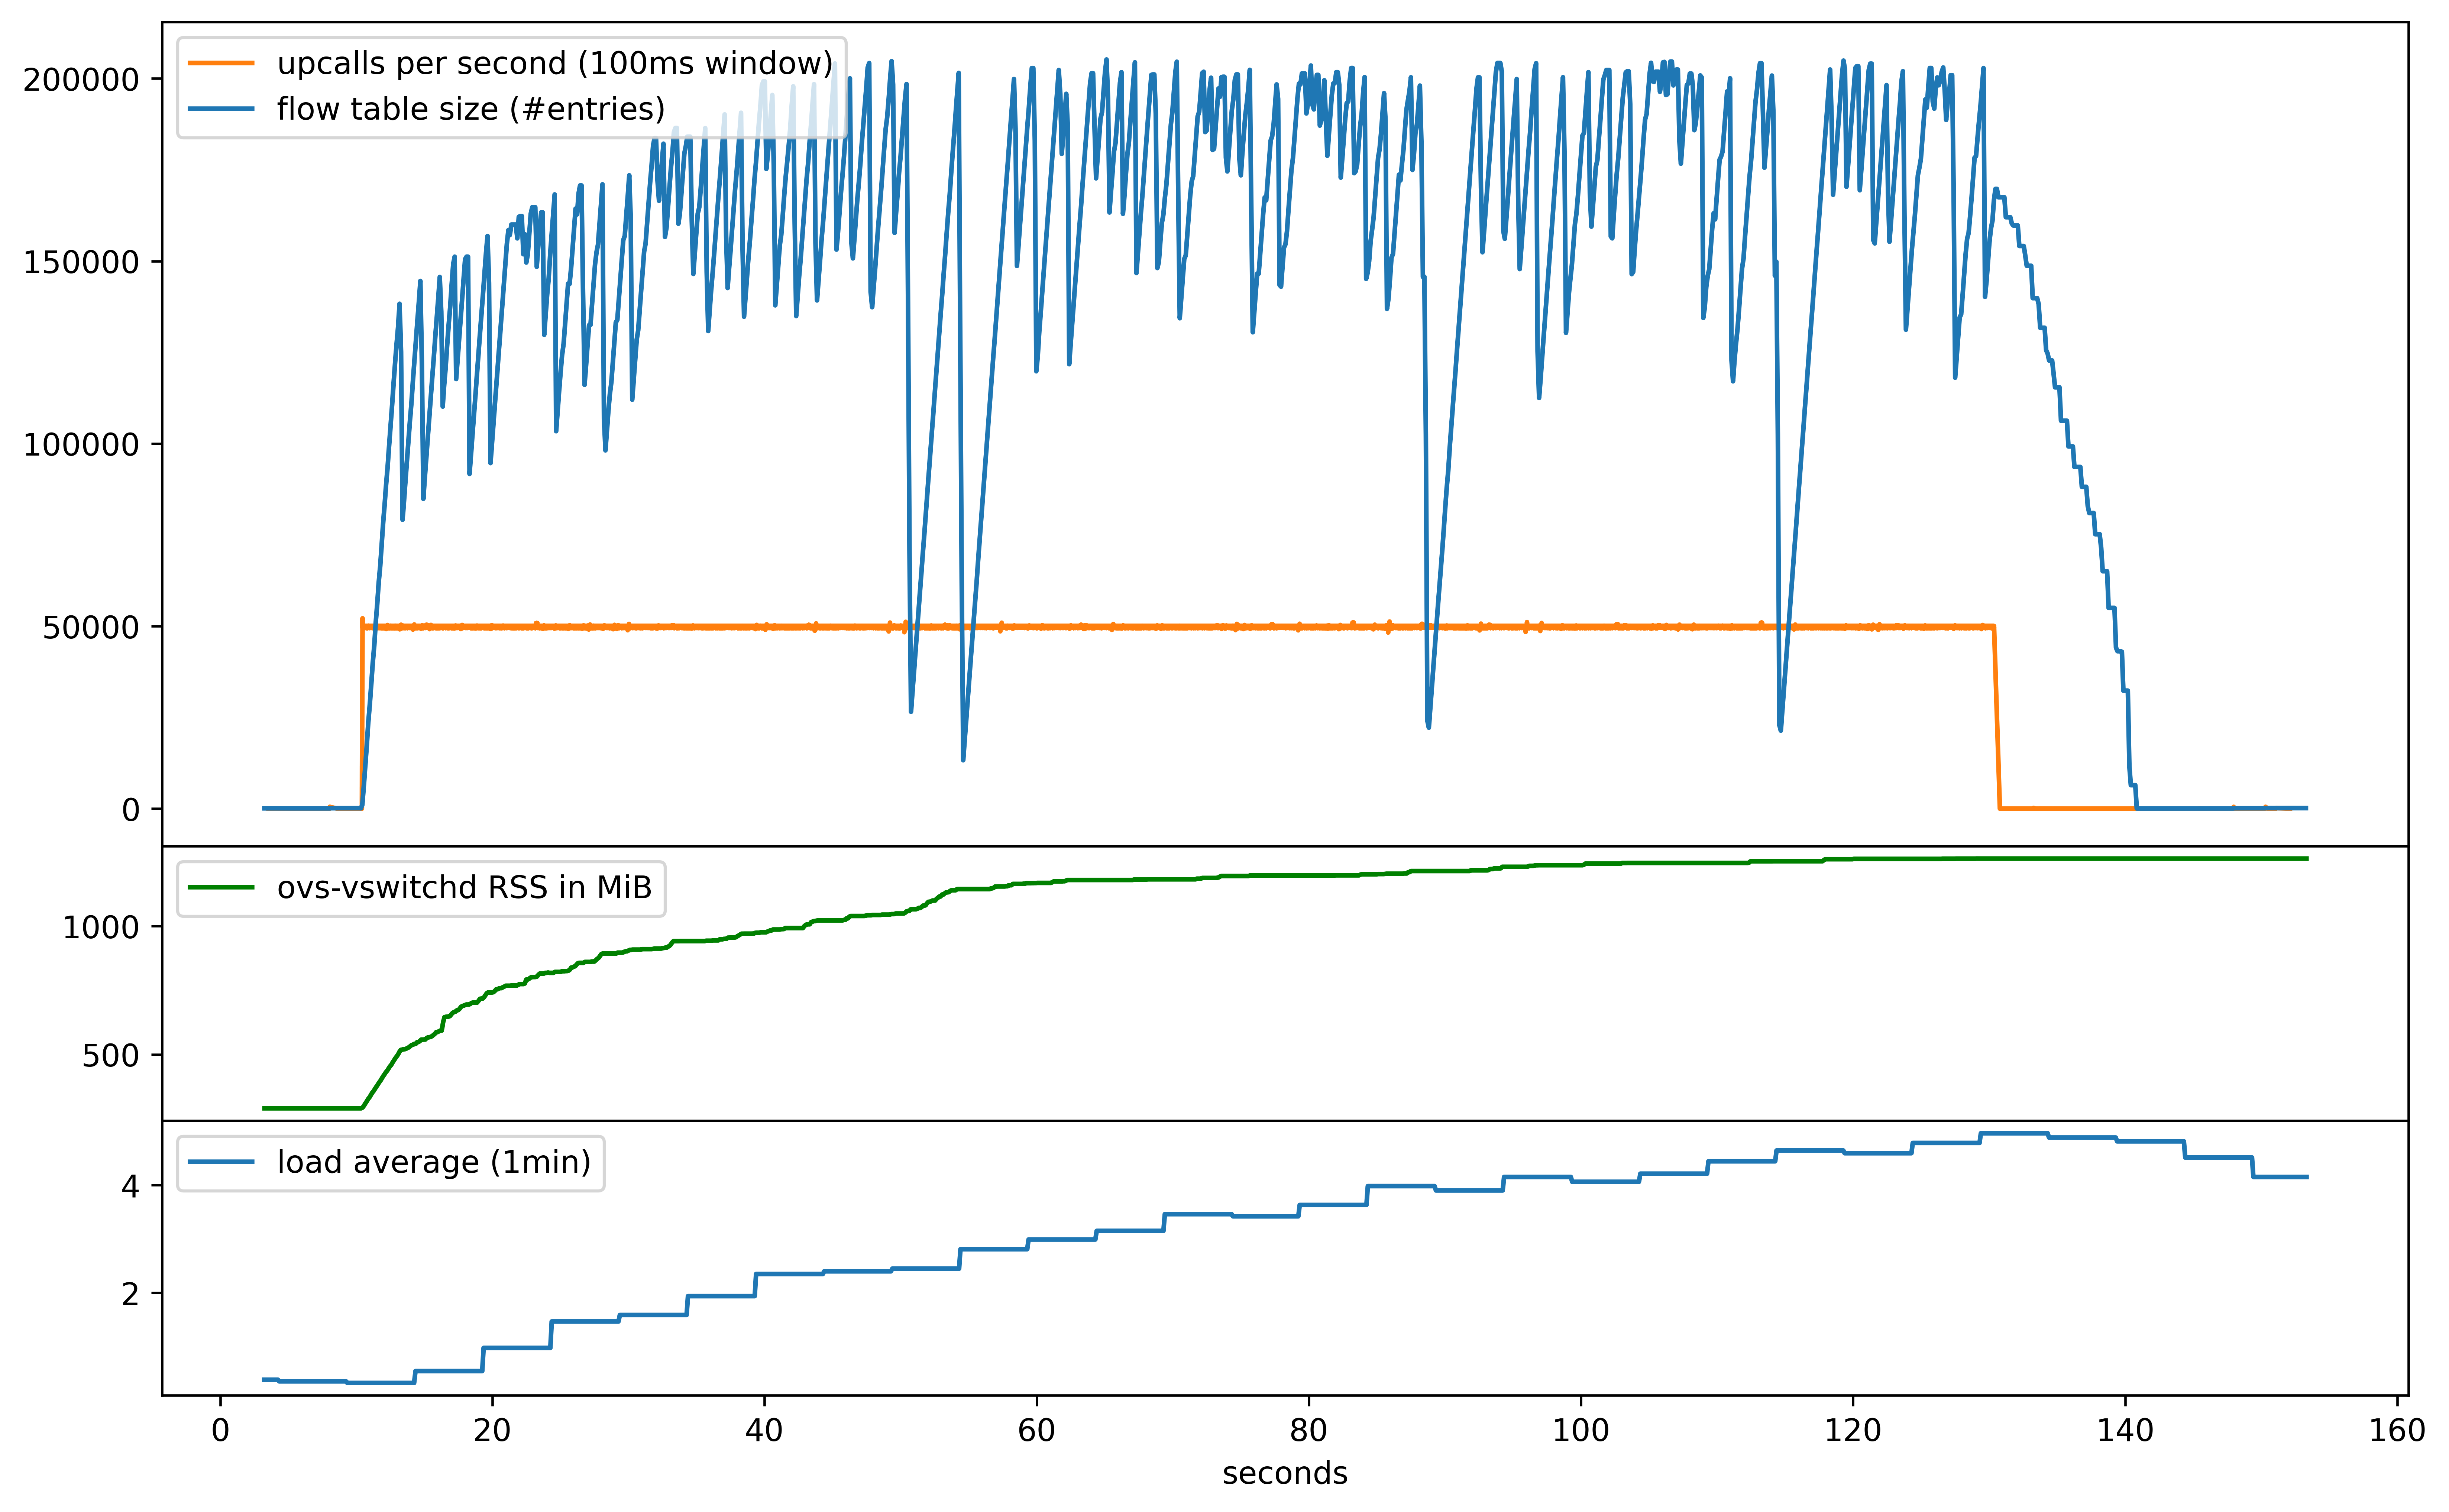
\includegraphics[width=.9\linewidth]{img/packet_flood_bare_50k.png}
    \caption{\ident{ovs-vswitchd} stressed with 50k upcalls per second}
    \label{fig:plot-packet-flood-bare-50k}
\end{figure}

\begin{figure}
    \centering
    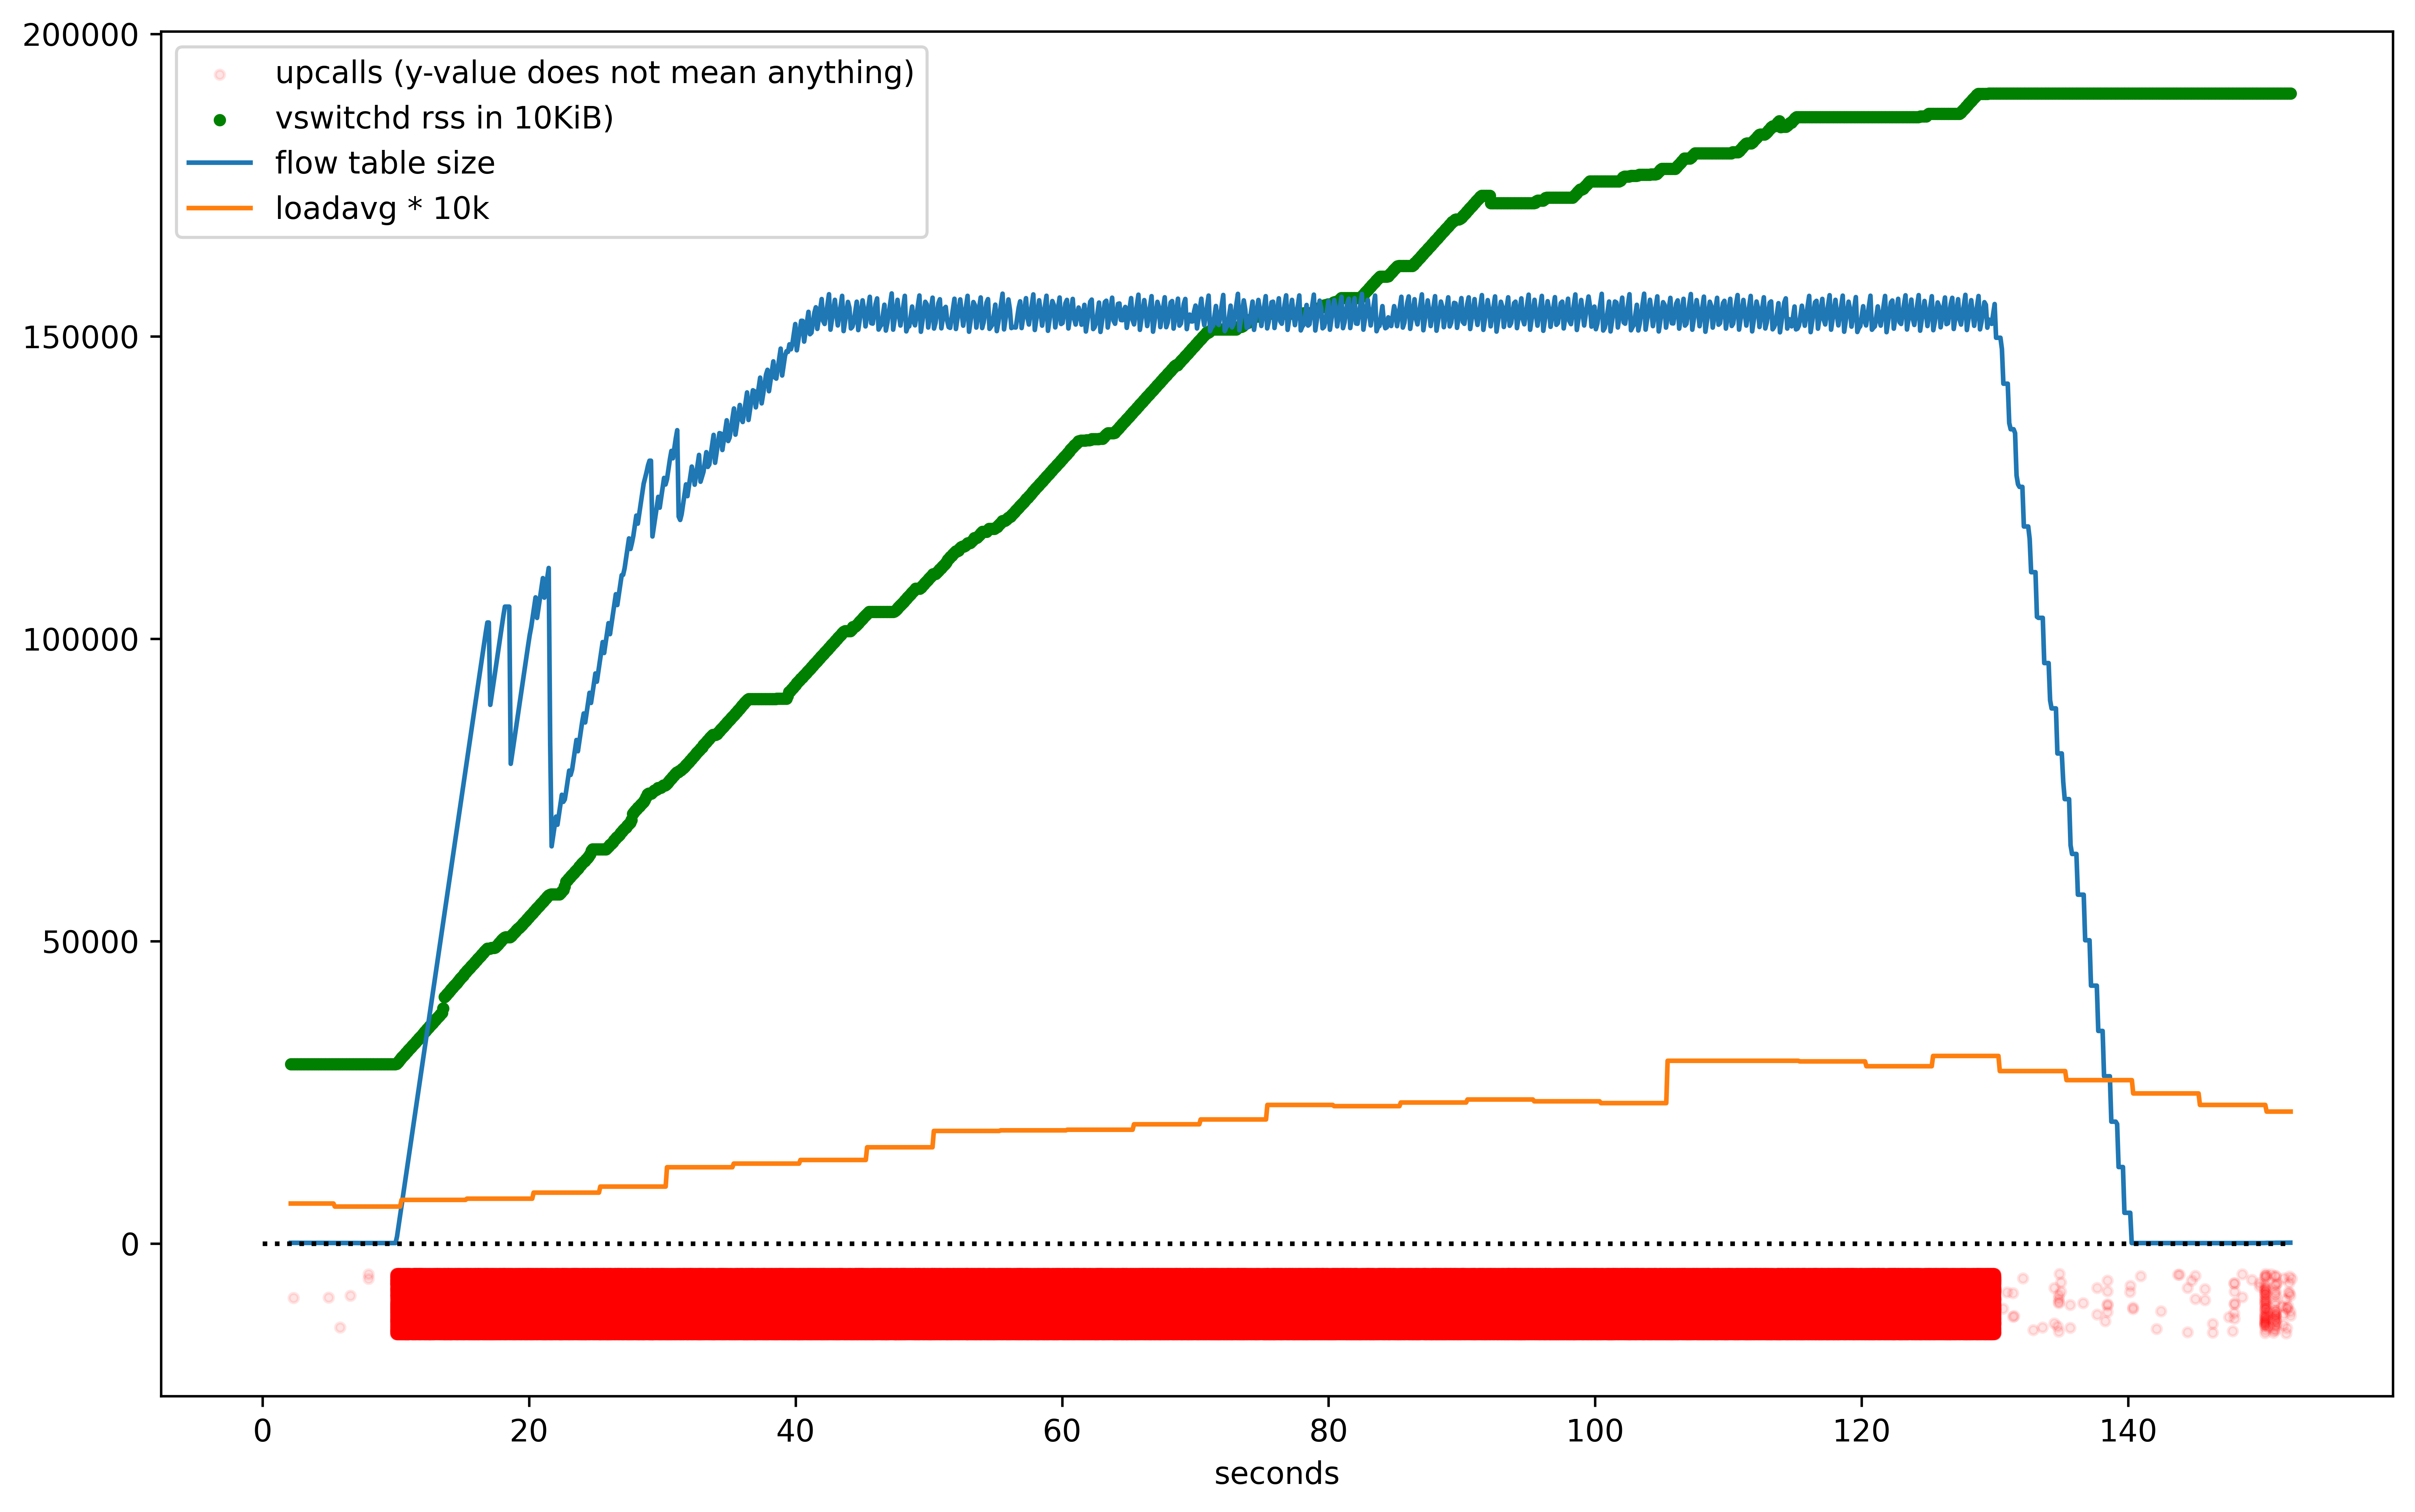
\includegraphics[width=.9\linewidth]{img/packet_flood_bare_15k.png}
    \caption{\ident{ovs-vswitchd} stressed with 15k upcalls per second}
    \label{fig:plot-packet-flood-bare-15k}
\end{figure}

\paragraph{Flow table size}
\Cref{fig:plot-packet-flood-bare-50k} and \cref{fig:plot-packet-flood-bare-15k} show recorded behavior of \ident{ovs-vswitchd} when stressed with significant number of upcalls. Assuming the 10-second flow rule timeout would be the only criteria for evicting flow rules, the flow tables should have reached 500k and 150k flow rules respectively. However, \ident{ovs-vswitchd} has a \href{https://github.com/openvswitch/ovs/blob/859071224c590207ca5e1f8723ffdef72ef7b512/ofproto/ofproto.h\#L310}{default limit of 200k flow rules} in the flow table which explains the lower-than-expected table size in \cref{fig:plot-packet-flood-bare-50k}. Moreso, the flow table size limit is dynamic based on measured system performance (more detail in \cref{subsec:cpu-limit}) and 200k is only a hard limit beyond which the table will never grow. The dynamic increase of the flow limit until the hard limit is reached is visible at the beginning of \cref{fig:plot-packet-flood-bare-50k}.

In both experiments, the flow table size fluctuates. With fewer upcalls, when only the timeout is at play, the fluctuations are small and can be explained by periodic timeout enforcement in the revalidator threads in \ident{ovs-vswitchd}. When the flow table size hits the 200k limit, an additional regulatory mechanism in the revalidator threads activates. Quoting a comment\footnote{\url{https://github.com/openvswitch/ovs/blob/474a179aff6c4199d8007910e3f79f000af9d659/ofproto/ofproto-dpif-upcall.c\#L2771-L2782}} from OVS's source code:

\begin{quote}
    In normal operation we want to keep flows around until they have
    been idle for 'ofproto\_max\_idle' milliseconds.  However:

    \begin{itemize}
        \item If the number of datapath flows climbs above 'flow\_limit', drop that down to 100 ms to try to bring the flows down to the limit.

        \item If the number of datapath flows climbs above twice 'flow\_limit', delete all the datapath flows as an emergency measure.  (We reassess this condition for the next batch of datapath flows, so we will recover before all the flows are gone.)
    \end{itemize}
\end{quote}

In other words, the revalidator thread checks flow rules in batches and whenever the flow table grows above the limit, a shorter eviction timeout is applied to the current batch. We hypothesize that the high amplitude of the fluctuations is caused by synchronization between multiple threads. There are multiple revalidator threads, each has its flow rule dump thread\footnote{\url{https://github.com/openvswitch/ovs/blob/474a179aff6c4199d8007910e3f79f000af9d659/ofproto/ofproto-dpif-upcall.c\#LL2751C16-L2751C16}} and the actual rule deletion is handled in the kernel after receiving a deletion command over a netlink socket which has an internal queue. We did not confirm nor disprove the hypothesis.

\paragraph{Upcalls}
In both \cref{fig:plot-packet-flood-bare-50k} and \cref{fig:plot-packet-flood-bare-15k}, the red dots at the bottom represent individual upcalls. We have randomized their position on the y-axis to improve legibility and better visualize upcall frequency.

Whenever our stress tool runs, the red bar becomes saturated and dense. Our tool tries to send packets in regular intervals, so the red bar should appear mostly homogeneous. At the end of the test, we report the results over the network and our tools are not perfectly synchronized, hence small upcall clusters at the end of the experiment are to be expected.

\paragraph{System load}
Because our packet flooding tool is a single-threaded application, it directly contributes to the load averages only by a value of 1 or less. However, we observe a significantly higher load average in both recorded experiments, in \cref{fig:plot-packet-flood-bare-50k} and in \cref{fig:plot-packet-flood-bare-15k}. Except for our running experiment, the system is idle. Hence we attribute the additional system load to OVS. As we discussed before in \cref{subsec:ovs-tasks}, OVS uses multiple threads during normal operation. By default, the revalidator threads iterate over the whole flow table every 500 \si{\milli\second} and command the kernel to delete flow rules. The upcall handlers continuously translate OpenFlow rules to datapath rules and command the kernel to insert new flow rules. All of this busy work causes the extra system load.

Worryingly though, the additional system load is not attributed to the process causing it. In Kubernetes, a container can have a resource limits \cite{KubernetesResourceManagement}. Flooding the system with upcalls from a resource-limited container would allow it to stress the system beyond its allowance. 

\paragraph{Memory usage}
\label{par:memory-usage}
In both \cref{fig:plot-packet-flood-bare-50k} and \cref{fig:plot-packet-flood-bare-15k}, the resident set size of \ident{ovs-vswitchd} increases and stabilizes at slightly less than 2GB. The allocated memory is never released and stays allocated even after the flooding stops. The used memory seems to be proportional to the flow table size.

Same as with the system load, memory usage bypasses resource accounting. A container or a VM with minimal resource allowance can use more resources than the system administrators configured.

\subsection{Impact on latency}

\begin{figure}
    \centering
    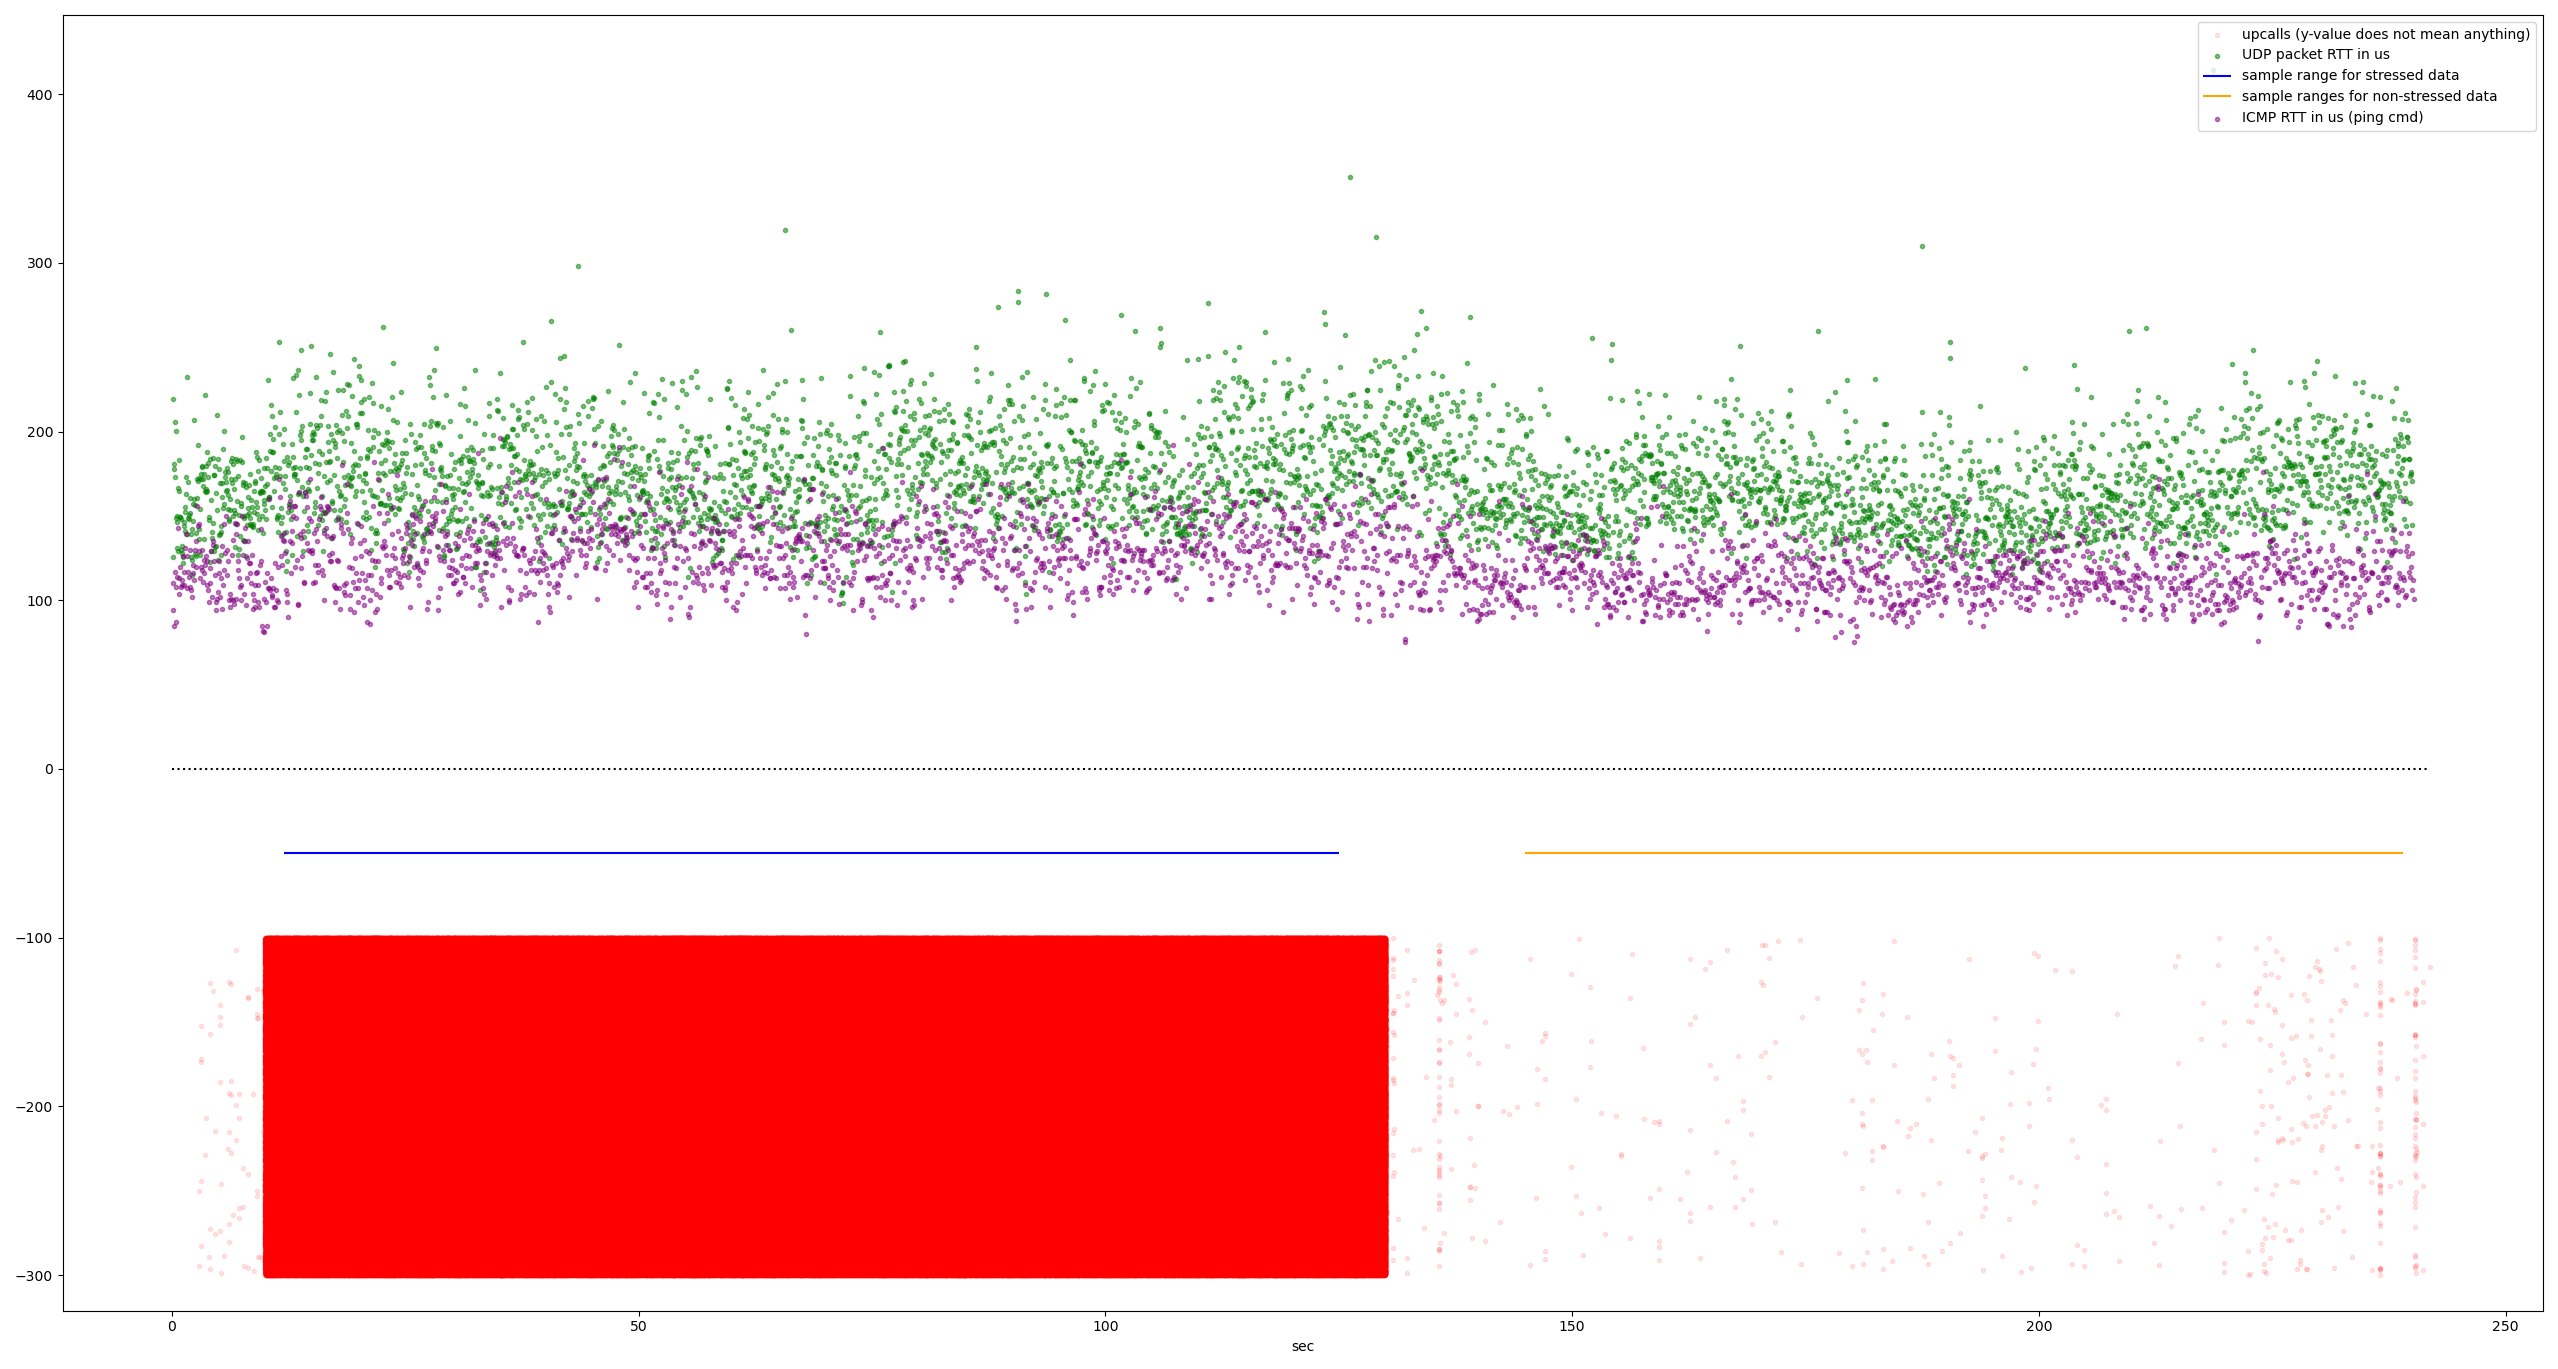
\includegraphics[width=.9\linewidth]{img/packet_flood_50k_latency.png}
    \caption{Round trip times during 50k upcalls/sec stress test}
    \label{fig:plot-packet-flood-50k-latency}
\end{figure}

\Cref{fig:plot-packet-flood-50k-latency} shows the results of a different run of the same experiment. The plot shows only the latencies measured from the \ident{victim} pod. The ICMP tests target the node IP address of \kb{1}, and the UDP tests target the node IP address of \kb{3}. The horizontal lines mark the ranges of samples used for a statistical test.

While there does not seem to be any practically significant difference between the stressed and non-stressed systems in the round-trip times, the difference is statistically significant. Considering only the UDP-based results, there are $2255$ samples in the stressed range with a mean value of $175980 \pm 1320$ \si{\nano\second}\footnote{$95\%$ confidence interval, assuming normal distribution}. The non-stressed range has 1876 samples and a mean value of $164404 \pm 1174$ \si{\nano\second}. The difference between the means is $11576$ \si{\nano\second}.

% stressed UDP latency
% shape: (9, 3)
% ┌────────────┬────────────┬───────────────┐
% │ describe   ┆ ts         ┆ latency_ns    │
% │ ---        ┆ ---        ┆ ---           │
% │ str        ┆ f64        ┆ f64           │
% ╞════════════╪════════════╪═══════════════╡
% │ count      ┆ 2255.0     ┆ 2255.0        │
% │ null_count ┆ 0.0        ┆ 0.0           │
% │ mean       ┆ 68.502237  ┆ 175980.142794 │
% │ std        ┆ 32.628849  ┆ 31963.391742  │
% │ min        ┆ 12.025217  ┆ 98250.0       │
% │ max        ┆ 124.979466 ┆ 762959.0      │
% │ median     ┆ 68.502056  ┆ 173259.0      │
% │ 25%        ┆ 40.238689  ┆ 155156.0      │
% │ 75%        ┆ 96.765862  ┆ 193006.0      │
% └────────────┴────────────┴───────────────┘
% (175980.14279379157, 174660.18226166346, 177300.10332591968)
% non-stressed UDP latencies
% shape: (9, 3)
% ┌────────────┬────────────┬───────────────┐
% │ describe   ┆ ts         ┆ latency_ns    │
% │ ---        ┆ ---        ┆ ---           │
% │ str        ┆ f64        ┆ f64           │
% ╞════════════╪════════════╪═══════════════╡
% │ count      ┆ 1876.0     ┆ 1876.0        │
% │ null_count ┆ 0.0        ┆ 0.0           │
% │ mean       ┆ 191.99893  ┆ 164404.665245 │
% │ std        ┆ 27.143008  ┆ 25925.644717  │
% │ min        ┆ 145.023486 ┆ 107262.0      │
% │ max        ┆ 238.975234 ┆ 495776.0      │
% │ median     ┆ 191.999098 ┆ 161704.5      │
% │ 25%        ┆ 168.52374  ┆ 146410.0      │
% │ 75%        ┆ 215.52409  ┆ 178624.0      │
% └────────────┴────────────┴───────────────┘
% (164404.66524520254, 163230.7366655189, 165578.5938248862)


\section{Performance when resource limited}

In \cref{subsec:standard-behavior}, we talked about extra memory and CPU usage of /ident{ovs-vswitchd}. The default containerized deployment of OVN-Kubernetes limits\footnote{https://github.com/ovn-org/ovn-kubernetes/blob/b982b8cadba939c55010829f61eb5ebe4fd90794/dist/templates/ovs-node.yaml.j2\#L84-L90} \ident{ovs-vswitchd} to 400 MiB of physical memory and two-tenths of a single CPU core. In the remainder of this section, when we write about limiting memory or CPU, we mean using Kubernetes to enforce the resource limit just as the default containerized deployment does it.

\subsection{Memory limit}
\label{subsec:memory}
We limited the memory usage of \ident{ovs-vswitchd}, leaving the CPU time unlimited. We used the default values for the memory limit, leaving us with the following configuration of the OVS container:

\begin{verbatim}
resources:
    requests:
        memory: 300Mi
    limits:
        memory: 400Mi
\end{verbatim}

When we flooded the system with upcalls, \ident{ovs-vswitchd} crashed without leaving any meaningful error message behind. During normal operations, everything seemed normal.

We tried to limit the number of flow rules using the following command:
\begin{verbatim}
ovs-vsctl set Open_vSwitch . other_config:flow-limit=10000
\end{verbatim}

The limit helps and when the upcall frequency is not too high (double or triple the limit), everything works. However, once we flood the network with even more packets, the flow limit is overshot and \ident{ovs-vswitchd} again crashes.

Our theory is that the crash happens during the revalidator dump phase, when \ident{ovs-vswitchd} makes a copy of all in-kernel flow rules in the userspace. This allocates more memory than allowed and the container is subsequently terminated by the OOM killer. Quoting Kubernetes Documentation \cite{KubeMemoryLimits}:

\begin{quote}
    A Container can exceed its memory request if the Node has memory available. But a Container is not allowed to use more than its memory limit. If a Container allocates more memory than its limit, the Container becomes a candidate for termination. If the Container continues to consume memory beyond its limit, the Container is terminated. If a terminated Container can be restarted, the kubelet restarts it, as with any other type of runtime failure.
\end{quote}

The decreased flow limit in the configuration of OVS does not help much to prevent crashes, because we can inject too many flows in between the revalidator thread runs (we can inject about 100k flow rules in 500ms, \ident{ovs-vswitch} crashes even with less).

\subsection{CPU limit}
\label{subsec:cpu-limit}

When CPU bound, \ident{ovs-vswitchd} does not crash. It tries to do the opposite and \href{https://github.com/openvswitch/ovs/blob/e3ba0be48ca457ab3a1c9f1e3522e82218eca0f9/ofproto/ofproto-dpif-upcall.c\#L1031-L1041}{dynamically changes the datapath's flow rule limit} based on the revalidator thread's performance:

\begin{verbatim}
duration = MAX(time_msec() - start_time, 1);
udpif->dump_duration = duration;
if (duration > 2000) {
    flow_limit /= duration / 1000;
} else if (duration > 1300) {
    flow_limit = flow_limit * 3 / 4;
} else if (duration < 1000 &&
            flow_limit < n_flows * 1000 / duration) {
    flow_limit += 1000;
}
flow_limit = MIN(ofproto_flow_limit, MAX(flow_limit, 1000));
\end{verbatim}

We can see the effect of this code in \cref{fig:packet-flood-limited}. The red dots (not upcalls) signify the dynamic flow limit. The horizontal lines going to the left of the dots signify the time the revalidator run took. We can see that a long revalidator run leads to a decreased flow limit.

% QT_QPA_PLATFORM=xcb python postprocessing/packet_flood.py results/packet_flood_2023-06-11T21:15+02:00/
\begin{figure}
    \centering
    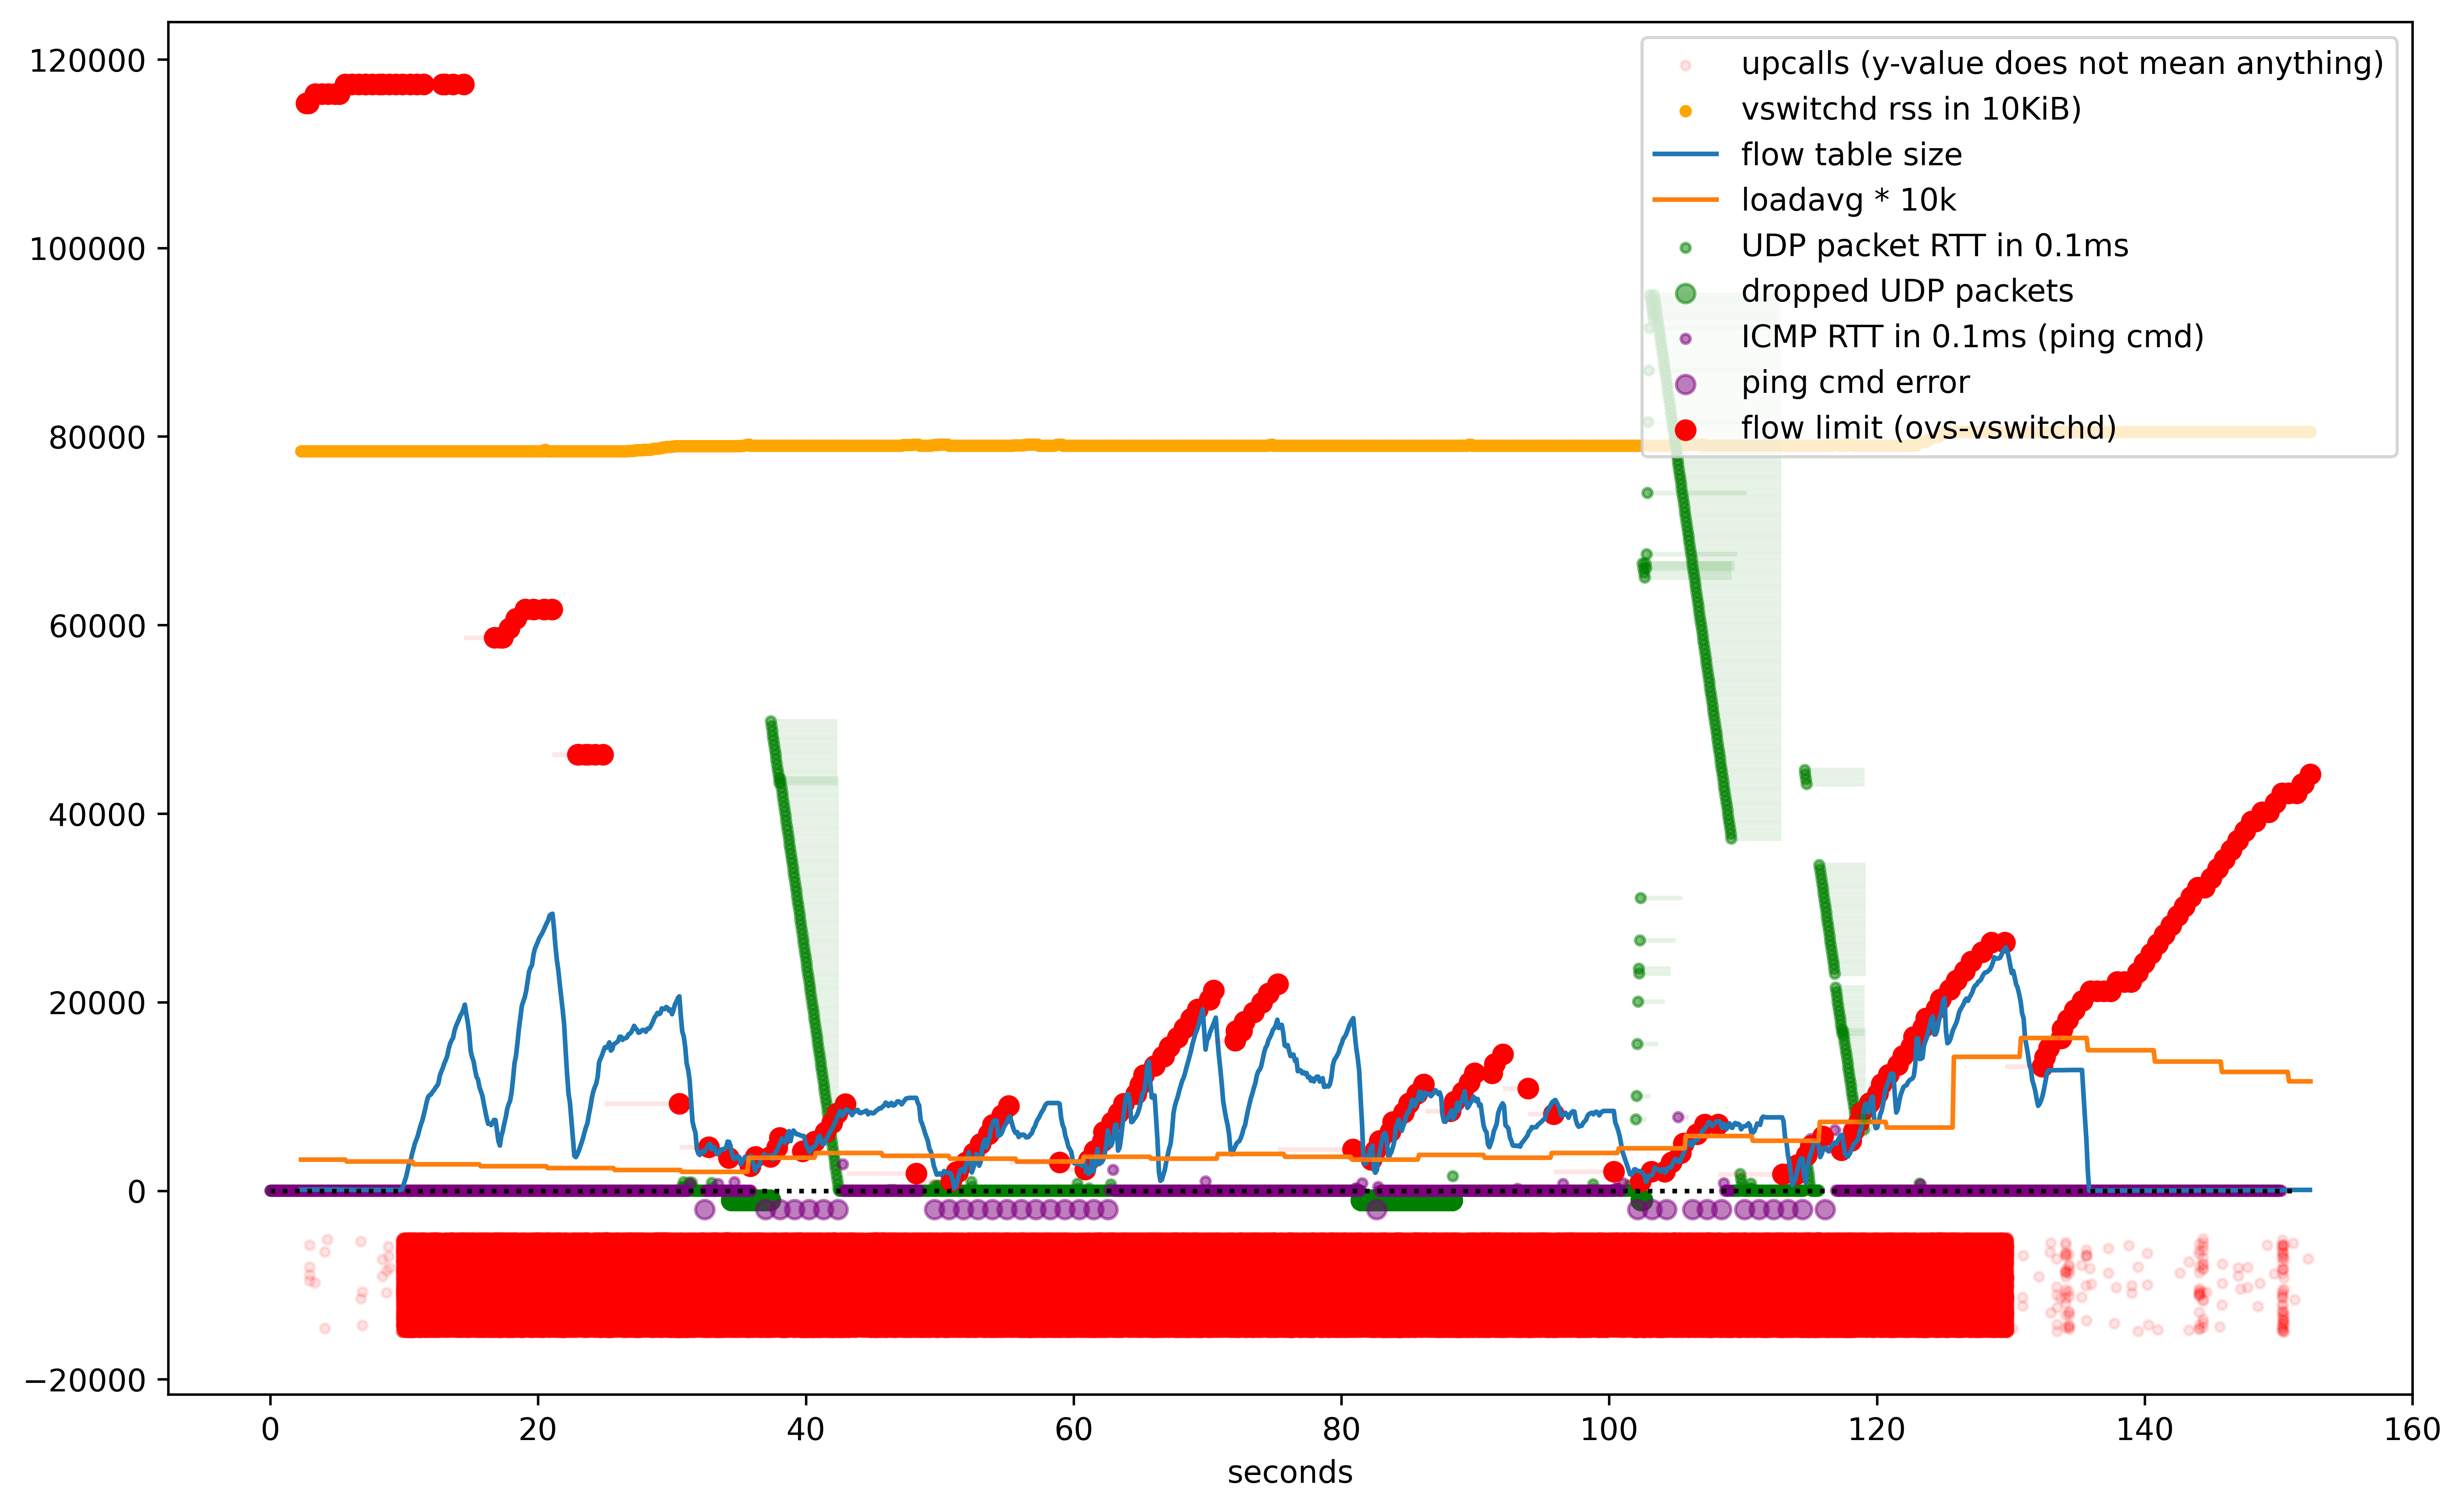
\includegraphics[width=.9\linewidth]{img/packet_flood_limited_resources_50k.png}
    \caption{5k upcalls/sec stress test}
    \label{fig:packet-flood-limited}
\end{figure}

 When compared to the previous experiments:

\begin{itemize}
    \item The rate of upcalls is only $5000$ per second, one-tenth of the experiments before.
    \item Memory usage stays almost constant.
    \item Load average (1 minute) peaks at the value 2, but stays below 1 most of the time.
    \item The size of the datapath flow table varies a lot more. We can see the same higher frequency variations as before, but now they are combined with lower frequency variations created by the dynamically changing flow limit.
    \item Latency measurements are added to the plot (beware of the unusual units). The measurement method is the same as when we talked about latency before, now combined into a single experiment. The highest round-trip time observed is around 10 seconds long. Sometimes, sending a packet completely fails (indicated by thicker dots below the number line). The lines signify when the packet was in-flight.
\end{itemize}

The extremely high round-trip times can be explained by the upcall buffer queues. When the revalidator threads and other tasks use most of the available resources, the handler threads might not get scheduled and the packets in upcalls are buffered until the handler threads run again. This explains the regular packet delivery pattern (the green diagonal lines on the plot). They are caused by a regular packet-sending interval and a single instant when all the packets are delivered in one big batch.

\paragraph{Flood with 200k packets per second}
When we send 200k packets per second (close to the limit of our tool's single-threaded performance), \ident{ovs-vswichd} does not crash, but no network traffic is getting through. The \ident{victim} pod on the same host was unable to receive any packet.

Interestingly, when we stop the stress test, the number of flow rules still oscillates for a couple of seconds before dropping to normal levels. This indicates that our hypothesis about queues in front of the handler threads was correct and that there are a lot of packets queued for processing. 

\subsection{CPU and memory limit}

When we use the default configuration with both CPU and memory limits, \ident{ovs-vswitchd} is still killed by OOM killer under extreme stress (200k upcall generating packets per second), even though the memory usage stays below the limit most of the time. The crashes are however not reliable and sometimes, \ident{ovs-vswitchd} runs normally for a while. The problem seems to be caused by a race condition between the flow limit calculation in revalidator threads and the handler threads inserting new flow rules. The crash happens when we change something - either at the beginning of a stress test or at the end, regardless of how long it is.

\subsection{Overloading \ident{ovs-vswitchd} without resource limits}

The crashes of \ident{ovs-vswitchd} led us to search for a possibility of a crash when overloaded without resource constraints. We tried to spawn multiple instances of our packet flooding tool, intentionally more threads than we had CPU cores available. On the 28-core dedicated test servers, we did not manage to crash \ident{ovs-vswitchd} with anywhere between 1 and 80 instances of our stress tool.

We believe that \ident{ovs-vswitchd} is safe from crashes as long as it runs without resource constraints. On our experimental clusters, \ident{ovs-vswitchd} is automatically configured as a higher priority process than the ordinary processes and therefore it gets enough CPU time. But even if we manually decrease the priority to the same level or below ordinary processes, \ident{ovs-vswitchd} does not crash.
%\chapter{Notable accidental discoveries and dead-ends}
\label{chap:accidents}

\xxx{This chapter might not be included in the final version. Now it's just a placeholder with a dump of random information. If you are reviewing my work, please jump straight away to the next chapter.}

\section{Accidental bug discovery}
\todo{this is really a placeholder with the email I wrote, replace it with something meaningful...}

Hi,

I think I might have found a bug or just a really weird unexpected behavior. I am reporting it here, but I've reproduced it only on systems with OVN-Kubernetes and OVN. I don't know whether it can be replicated with standalone OVS.


\subsection{Test environment}


3 node Kubernetes cluster using OVN-Kubernetes, Docker and Fedora 38. All nodes in a single LAN with IPs 192.168.1.{221,222,223}. From now on, I will refer to the nodes only by the last digit of their IP address.


\subsection{Steps to reproduce:}


\begin{enumerate}
\item install a pod with a shell and a ping command (I am using docker.io/archlinux:latest, always running on node 222)
\item run `kubectl exec -ti \$POD\_NAME -- ping 192.168.1.221`
\item in a different terminal, ssh into the host of the pod (in my case node 222) and run `ovs-dpctl del-flows`
\item observe the measured latencies
\item keep the ping running and kill ovs-vswitchd on the host and wait for its restart
\item observe the latencies
\end{enumerate}


\subsection{What I observe}


\begin{verbatim}
[root@wsfd-netdev64 ~]# kubectl exec -ti arch -- ping 192.168.1.221
PING 192.168.1.221 (192.168.1.221) 56(84) bytes of data.
64 bytes from 192.168.1.221: icmp_seq=1 ttl=63 time=0.543 ms
64 bytes from 192.168.1.221: icmp_seq=2 ttl=63 time=0.160 ms
64 bytes from 192.168.1.221: icmp_seq=3 ttl=63 time=0.119 ms
64 bytes from 192.168.1.221: icmp_seq=4 ttl=63 time=0.144 ms
64 bytes from 192.168.1.221: icmp_seq=5 ttl=63 time=0.137 ms
64 bytes from 192.168.1.221: icmp_seq=6 ttl=63 time=0.996 ms  # < ovs-dpctl del-flows
64 bytes from 192.168.1.221: icmp_seq=7 ttl=63 time=0.808 ms
64 bytes from 192.168.1.221: icmp_seq=8 ttl=63 time=1.01 ms
64 bytes from 192.168.1.221: icmp_seq=9 ttl=63 time=1.24 ms
64 bytes from 192.168.1.221: icmp_seq=10 ttl=63 time=1.20 ms
64 bytes from 192.168.1.221: icmp_seq=11 ttl=63 time=1.14 ms
64 bytes from 192.168.1.221: icmp_seq=12 ttl=63 time=1.10 ms  # < killall ovs-vswitchd
  From 10.244.1.5 icmp_seq=22 Destination Host Unreachable
  From 10.244.1.5 icmp_seq=23 Destination Host Unreachable
  From 10.244.1.5 icmp_seq=24 Destination Host Unreachable
  From 10.244.1.5 icmp_seq=25 Destination Host Unreachable
  From 10.244.1.5 icmp_seq=26 Destination Host Unreachable
  From 10.244.1.5 icmp_seq=27 Destination Host Unreachable
  From 10.244.1.5 icmp_seq=28 Destination Host Unreachable
  From 10.244.1.5 icmp_seq=29 Destination Host Unreachable
  From 10.244.1.5 icmp_seq=31 Destination Host Unreachable
  From 10.244.1.5 icmp_seq=32 Destination Host Unreachable
64 bytes from 192.168.1.221: icmp_seq=34 ttl=63 time=1371 ms
64 bytes from 192.168.1.221: icmp_seq=35 ttl=63 time=322 ms
64 bytes from 192.168.1.221: icmp_seq=36 ttl=63 time=0.186 ms
64 bytes from 192.168.1.221: icmp_seq=37 ttl=63 time=0.192 ms
64 bytes from 192.168.1.221: icmp_seq=38 ttl=63 time=0.140 ms
64 bytes from 192.168.1.221: icmp_seq=39 ttl=63 time=0.163 ms
^C
--- 192.168.1.221 ping statistics ---
39 packets transmitted, 18 received, +10 errors, 53.8462% packet loss, time 38769ms
rtt min/avg/max/mdev = 0.119/94.570/1370.551/318.102 ms, pipe 3
\end{verbatim}

After flushing the datapath flow rules, the RTTs increase. This indicates an upcall for every single packet. I confirmed this by tracing the kernel and the upcalls are definitely there (actually, this is how I discovered the whole issue). The system can remain in this state for a long time (at least minutes).

After restarting vswitchd, the upcalls stop happening and everything is fast again.


I have also confirmed, that the same thing happens to UDP packets. The same also happens regardless of which node in the cluster I target, even the pod's host.


\subsection{What I expect}


I expected only a few upcalls in response to flushing the datapath, after which a new datapath rules would get inserted into the kernel.


\subsection{Repeatability}


Flushing the rules and restarting vswitchd seems to be a certain method to flip the system between the two different states. However the upcall-making state seems unstable and it sometimes reverts back to the expected lower-latency state by itself. It appears to me that flooding the system with unrelated upcalls and rules increases the chance of an "autonomous fix".


At this point, I don't believe this would cause significant problems. I just find the behavior extremely weird.

Is there something more I could provide to help with reproducing this? Or should I report it elsewhere?


Best,
Vašek Šraier 

\section{Lock contention investigation}
\todo{write about the fact, that there does not seem to be a problematic lock in OVS, because we checked them almost all}



\chapter{Discussion}
\label{chap:discussion}
\todo{hmm, is there something to write here?}

\section{List of open question}
\todo{what are the things we found and do not know the answer to?}


\section{Improvement suggestions}
\todo{What can be made better about OVS, OVN, OVN-Kubernetes}



\chapwithtoc{Conclusion}

In the conclusion, you should summarize what was achieved by the thesis. In a few paragraphs, try to answer the following:
\begin{itemize}
\item Was the problem stated in the introduction solved? (Ideally include a list of successfully achieved goals.)
\item What is the quality of the result? Is the problem solved for good and the mankind does not need to ever think about it again, or just partially improved upon? (Is the incompleteness caused by overwhelming problem complexity that would be out of thesis scope\todo{This is quite common.}, or any theoretical reasons, such as computational hardness?)
\item Does the result have any practical applications that improve upon something realistic?
\item Is there any good future development or research direction that could further improve the results of this thesis? (This is often summarized in a separate subsection called `Future work'.)
\end{itemize}


\ifEN
\chapwithtoc{Bibliography}
\else
\chapwithtoc{Seznam použité literatury}
\fi

\printbibliography[heading=none]


\appendix
\chapter{\ident{ovs-vswitchd} container image}
\label{chap:ovs-mod}

\section{Build}

There is a script \ident{build\_ovs\_container.sh} attached to this thesis. Running this script will download and compile OVS, OVN and OVN-Kubernetes and at the end, wrap the result into a container usable for deployment into a cluster. We recommend reading the script first before running it. It is not long and it might be desirable to tweak it.

To run the script, make sure that you have these dependencies installed on your system:

\begin{itemize}
    \item \ident{podman}, ideally configured for rootless operation
    \item \ident {git}
    \item \ident{go} compiler
\end{itemize}

The script creates a container image by default called \ident{ovn-kube-f:latest}. To use it further in the cluster, push it to an accessible container registry\footnote{We run a private registry for this purpose.} and note its fully qualified name.

\section{Our changes to OVS}

All changes we have made to OVS can be seen in the \ident{ovs-usdt-probes.patch} file. We have added only new USDT probes. They are compiled only as \ident{nop} instructions and should not significantly impact the performance unless used.

\chapter{Cluster installation instructions}
\label{chap:install}

Start by preparing 3 standard Fedora 38 installations, all in a single LAN, ideally with 2 network cards as described in \cref{sec:hw-env}. All systems should have an accessible root shell. Any time we write about running a command, we always assume it is run from the root shell.

In the attachment, there are two scripts prefixed with \ident{setup}. First, we advise editing both of the scripts:

\begin{itemize}
    \item Edit the \ident{setup1-general.sh} script and change the network configuration function, \ident{configure\_systemd\_networkd}, to match your network environment. Especially the names of your network interfaces.

    \item Edit the \ident{setup2-master.sh} script and change \ident{\$IMAGE} variable with the qualified name of your OVS container (instructions on how to build it in \cref{chap:ovs-mod}).
\end{itemize}

Once you changed the script, follow these steps:

\begin{enumerate}
    \item Run the \ident{setup1-general.sh} script on all machines. Provide \kb{1}, \kb{2} or \kb{3} as an argument to set the hostnames.

    \item Wait for all the systems to reboot.

    \item On the machine you chose as \kb{1}, run the \ident{setup2-master.sh} script.

    \item On \kb{1}, run \ident{kubeadm token create -{}-print-join-command}

    \item Append the \ident{-{}-cri-socket=unix:///var/run/cri-dockerd.sock} option at the end of the output of the previous step and run the command on both \kb{2} and \kb{3}.

    \item Wait for the cluster to initialize, i.e. the command \ident{kubectl get nodes} on \kb{1} should shows that all 3 nodes are in the \ident{Ready} state.

    \item Copy pod specification files from the \ident{kube\_configs} directory to \kb{1}. Edit the \ident{reflector.yaml} file and change the image reference to your build of the \ident{analyzer} container (see \cref{chap:analyzer}). Create the pods by calling \ident{kubectl create -f \$file}.

    \item Check the pods deployment status using \ident{kubectl get pods}. Make sure that all pods are in the \ident{Ready} state before proceeding.

    \item At this point, you can run the experiments. To get a root shell in the \ident{arch} pod, use the \ident{kubectl exec -ti arch -{}- /bin/bash} command. Similarly for the \ident{victim} pod.
\end{enumerate}
\chapter{\ident{analyzer} - the tool for running experiments}
\label{chap:analyzer}

\section{Build}

The source code is located in the \ident{analyzer} directory in the attachment. Only the Rust toolchain is required for compilation:

\begin{verbatim}
# in the analyzer/ directory
cargo build --release --target=x86_64-unknown-linux-musl
# the executable will be located at 
#    analyzer/target/x86_64-unknown-linux-musl/release/analyzer
\end{verbatim}

Continue by building the container image:

\begin{verbatim}
# again in the analyzer/ directory
podman build -t analyzer .
\end{verbatim}

Push the image to your container registry of choice and remember the qualified container name. The image is required for the \ident{reflector} pod, more in \cref{chap:install}. Also, copy the binary to the \ident{\$PATH} on all nodes and pods.

\section{Usage}

The \ident{analyzer} is generally a collection of smaller tools, all invoked via subcommands. The tool can be always supplied with the \ident{-{}-help} option and it will print out a help message. The following subsections will describe how to use the \ident{analyzer} for the discussed experiments.

\paragraph{Data collection} The measurement results are stored in files in the \ident{analyzer}'s current working directory. Multiple files are usually created. The file names start with a human-readable identifier of the data series. The second part of the file names is a timestamp (identical for all files created in a single \ident{analyzer} run).

The \ident{analyzer} can upload results to an HTTP server when provided with the \ident{-{}-push-results-url} argument. When the URL is provided, for every data file it creates, the \ident{analyzer} calls the \ident{curl -T [FILE] \{URL\}} command. 

\paragraph{Data format}

The result files are usually using the CSV format. All data series use the same time source (see \cref{subsec:clock}). Therefore, all measurements can be easily aligned even when the collected data came from different \ident{analyzer} runs (i.e. in a pod and on a host at the same time).

\subsection{Eviction timeout measurement}

The result of this experiment is a single CSV file with timestamps and the measured round-trip times.

\begin{verbatim}
# on arch (pod)
analyzer randomized-eviction-timeout \
		--target-ip 192.168.1.221 \
		--count 3
\end{verbatim}

\subsection{Packet fuzzing}

This experiment creates multiple data files, not all of which are relevant. From the \ident{node-logger} subcommand, we are interested in upcall statistics located in the \ident{kernel\_flow\_table\_trace*.csv} file. The \ident{tags*.jsonl} file from the \ident{packet-fuzz} subcommand provides us with timestamps allowing us to separate the upcalls into categories.

\begin{verbatim}
# on kb2
analyzer install-dependencies
analyzer node-logger --only-upcalls

# on arch (pod)
analyzer install-dependencies
analyzer packet-fuzz
\end{verbatim}


\subsection{Packet flood}

In this experiment, we were not looking for anything in particular, therefore all the result files can be of interest.

\begin{verbatim}
# on arch (pod)
analyzer packet-flood --count 500000

# on victim (pod)
analyzer victim

# on kb2
analyzer install-dependencies
analyzer node-logger --only-upcalls
\end{verbatim}

\section{Processing of results}

Scripts for creating plots are located in the \ident{analyzer/postprocessing} directory. To use them, it is necessary to install Python, matplotlib, Polars, Pandas, numpy and scipy.

There is a script for every experiment type. The packet flood experiment has multiple similar scripts with slightly differently preconfigured plots, the others have only a single script. The scripts, especially the packet-flood related, contain extra commented-out code to plot additional data.

All scripts expect two arguments - a path to a directory containing all results from a single experiment and the name of the output file.

% if your attachments are complicated, describe them in a separate appendix
%\include{attachments}

\openright
\end{document}
